\documentclass[conference]{IEEEtran}
% Compile: pdflatex main.tex (twice) on Overleaf/TeX Live, or `tectonic main.tex`. Figures live in figures/.
\usepackage[T1]{fontenc}
\usepackage{amsmath,amssymb}
\usepackage{graphicx}
\usepackage{booktabs}
\usepackage{multirow}
\usepackage{xcolor}
\usepackage{tikz}
\usetikzlibrary{arrows.meta,positioning,fit,calc,shapes.geometric}
\usepackage[hidelinks]{hyperref}
\usepackage{url}
\graphicspath{{figures/}}
% let floats (especially full-width figure*) share pages with text instead of piling up at the end
\renewcommand{\topfraction}{0.9}\renewcommand{\dbltopfraction}{0.9}\renewcommand{\bottomfraction}{0.8}
\renewcommand{\textfraction}{0.07}\renewcommand{\floatpagefraction}{0.5}\renewcommand{\dblfloatpagefraction}{0.5}
\setcounter{topnumber}{3}\setcounter{dbltopnumber}{3}\setcounter{totalnumber}{5}

% ---- items the author must fill in before submission (shown in red until replaced)
\newcommand{\TODO}[1]{\textcolor{red}{\textbf{[#1]}}}
\newcommand{\authorname}{Abubakar}
\newcommand{\rollno}{23i0515}
\newcommand{\youtubeurl}{\TODO{YouTube link of the demo video}}
\newcommand{\repourl}{\url{https://github.com/Abubakar7-dotcom/Gen_ai_assignment1}}
\newcommand{\releaseurl}{\url{https://github.com/Abubakar7-dotcom/Gen_ai_assignment1/releases/tag/models-v1}}
\newcommand{\wandburl}{\url{https://wandb.ai/abubaknaveed-national-university-of-computer-and-emergi/genai-a1}}

\tikzset{
  blk/.style={draw, rounded corners=2pt, align=center, font=\scriptsize, inner sep=2.5pt, minimum height=5mm},
  enc/.style={blk, fill=blue!8},
  dec/.style={blk, fill=orange!10},
  lat/.style={blk, fill=green!12, thick},
  io/.style={blk, fill=gray!10},
  arr/.style={-{Stealth[length=1.6mm]}, thin},
}

\begin{document}

\title{Image Restoration with Autoencoders, Hard Routing and a Soft Mixture of Experts, and Style-Conditioned
Face-to-Sketch Generation with a Conditional GAN}

\author{\IEEEauthorblockN{\authorname}
\IEEEauthorblockA{Generative AI, Assignment 1 --- Roll No.\ \rollno, Section A\\
National University of Computer and Emerging Sciences (FAST-NUCES)\\
Code: \repourl}}

\maketitle

\begin{abstract}
We build and deploy four related generative systems. On the Oxford-IIIT Pet dataset, images corrupted at runtime
by salt-and-pepper noise, Gaussian blur or rectangular occlusion are restored by (1) a single universal denoising
autoencoder, (2) a corruption classifier that hard-routes each image to one of three specialist autoencoders or an
identity bypass, and (3) a jointly fine-tuned soft mixture of experts (MoE) whose gate blends the identity branch
and the three experts. On FS2K, (4) a pix2pix-style conditional GAN with a learned style embedding in both
generator and discriminator turns a face photograph into a sketch of one of three styles. Every task is tuned with
Optuna, tracked in Weights \& Biases, exported to ONNX (max.\ PyTorch--ONNX Runtime difference
$6.6\times10^{-6}$) and served by one React + FastAPI application started with a single
\texttt{docker compose} command. The classifier reaches 99.6\% accuracy (macro-F1 0.993) and the MoE gate routes
99.3\% of test images to the correct branch. Restoration quality is limited to about 23\,dB by the
compressed $8\times8$ latent code: removal of salt-and-pepper noise and occlusions improves PSNR by 6.5--7\,dB, but
blurred and clean inputs lose detail. An ablation shows that a single narrow skip connection raises validation
PSNR from 22.4 to 27.3\,dB, identifying the spatial bottleneck as the main limit.
\end{abstract}

\begin{IEEEkeywords}
denoising autoencoder, mixture of experts, conditional GAN, pix2pix, Optuna, ONNX, image restoration
\end{IEEEkeywords}

% =====================================================================================================
\section{Introduction}
Real images are degraded in different ways, and a restoration system usually does not know which degradation it
faces. This assignment studies three ways to handle several corruptions with the same budget of autoencoders: one
shared model for everything (Task~1), an explicit classifier that picks a specialist (Task~2), and a differentiable
gate that blends specialists (Task~3). Task~4 moves from restoration to paired image-to-image generation and asks
for a single generator that produces three distinct sketch styles. The four models are integrated into one
containerised browser application so that an evaluator can corrupt or upload unseen images and inspect the routing
decisions, weights and timings.

Our contributions are: a single corruption implementation shared by training, evaluation and the application
(Section~\ref{sec:data}); Optuna studies for all four tasks with documented search spaces
(Section~\ref{sec:setup}); per-condition and per-severity results with failure analysis for each task
(Sections~\ref{sec:t1}--\ref{sec:t4}); two ablations that explain the main weakness of the restoration models
(Section~\ref{sec:ablation}); and a deployment that is tested end to end from a fresh clone
(Section~\ref{sec:app}).

% =====================================================================================================
\section{Related Work}
\textbf{Denoising autoencoders.} Vincent \emph{et al.}~\cite{vincent2008,vincent2010} train an autoencoder to
reconstruct a clean input from a corrupted one, which forces the code to capture structure rather than copy pixels.
Restoration networks such as RED-Net~\cite{mao2016} and DnCNN~\cite{zhang2017} reach much higher fidelity by adding
symmetric skip connections or by predicting the residual, i.e.\ by letting the input bypass the bottleneck. The
assignment forbids unrestricted skips so that the latent code stays a genuine compression; Section~\ref{sec:ablation}
measures what this costs.

\textbf{Loss functions.} SSIM~\cite{wang2004} compares local luminance, contrast and structure. Zhao
\emph{et al.}~\cite{zhao2017} showed that an $\ell_1$ term combined with (MS-)SSIM gives better restorations than
$\ell_2$, which over-smooths; this motivates the $\alpha\,\ell_1 + (1-\alpha)(1-\mathrm{SSIM})$ loss used here.

\textbf{Mixtures of experts.} Jacobs \emph{et al.}~\cite{jacobs1991} introduced a gating network that softly assigns
inputs to experts. Sparsely-gated MoEs~\cite{shazeer2017} and Switch Transformers~\cite{fedus2022} add auxiliary
load-balancing losses because gates tend to collapse onto a few experts; our balance term follows the same idea.
Hard routing (Task~2) corresponds to a top-1 gate trained separately from the experts.

\textbf{Conditional GANs.} GANs~\cite{goodfellow2014} learn a generator through an adversarial discriminator;
conditional GANs~\cite{mirza2014} feed side information to both networks. Pix2pix~\cite{isola2017} combines a U-Net
generator~\cite{ronneberger2015}, a PatchGAN discriminator that judges local patches, and an $\ell_1$ term with
$\lambda=100$. FS2K~\cite{fan2022} provides photo--sketch pairs in three styles and benchmarks this kind of model;
earlier face-sketch work used exemplar-based synthesis~\cite{wang2009}.

\textbf{Tools.} Optuna~\cite{akiba2019} implements the Tree-structured Parzen Estimator (TPE)~\cite{bergstra2011}
and median pruning; Weights \& Biases~\cite{wandb} tracks runs; ONNX Runtime~\cite{onnxruntime} runs exported models
without PyTorch.

% =====================================================================================================
\section{Data and Corruption Pipeline}\label{sec:data}
\textbf{Oxford-IIIT Pet}~\cite{parkhi2012}. The official \texttt{trainval} list (3,680 images) is split 80/20 with
seed 42 into 2,944 training and 736 validation images; the 3,669 official test images are used only for the final
evaluation. Images are converted to RGB, resized to $128\times128$ (area interpolation) and cached once as a
\texttt{uint8} array; corrupted copies are never stored. The same split is used for Tasks~1--3.

\textbf{Runtime corruption.} One NumPy/OpenCV module implements the four conditions
(Table~\ref{tab:corruptions}) and is imported by training, manifest generation, evaluation and the FastAPI backend,
so the application behaves exactly like the reported experiments. During training every loaded image draws a new
condition and severity. A batch sampler gives every batch exactly $B/4$ images of each condition, which satisfies
the balanced-batch requirement deterministically. Occlusion coverage is measured as the area of the
\emph{union} of the rectangles and resampled until it lies in range, because summing rectangle areas over-counts
overlaps.

\textbf{Deterministic evaluation.} A validation manifest stores one condition per validation image (184 per
condition) and a test manifest stores, for each of the 3,669 test images, the clean version plus every corruption at
three fixed severities (36,690 items). Each entry records type, severity, parameters (probability, kernel and
$\sigma$, rectangle coordinates) and seed. Fig.~\ref{fig:sanity} shows samples.

\begin{table}[!htbp]
\centering\caption{Corruption configuration (training ranges and fixed test severities)}\label{tab:corruptions}
\scriptsize\setlength{\tabcolsep}{2.5pt}
\begin{tabular}{@{}lp{0.37\columnwidth}p{0.33\columnwidth}@{}}
\toprule
Condition & Training (runtime, uniform) & Test low / medium / high \\
\midrule
Clean & unchanged & --- \\
Salt \& pepper & $p\sim U(0.02,0.15)$; pixel set to black or white w.p.\ 0.5 & $p=0.03$ / $0.08$ / $0.15$ \\
Gaussian blur & $k\in\{3,5,7\}$, $\sigma\sim U(0.5,2.5)$ & $(k,\sigma)=(3,0.7)$ / $(5,1.5)$ / $(7,2.5)$ \\
Occlusion & 1--3 black rectangles, union area 10--35\%, random positions & 1 / 2 / 3 rectangles, $\approx$10 / 20 / 35\% \\
\bottomrule
\end{tabular}
\end{table}

\begin{figure*}[t]
\centering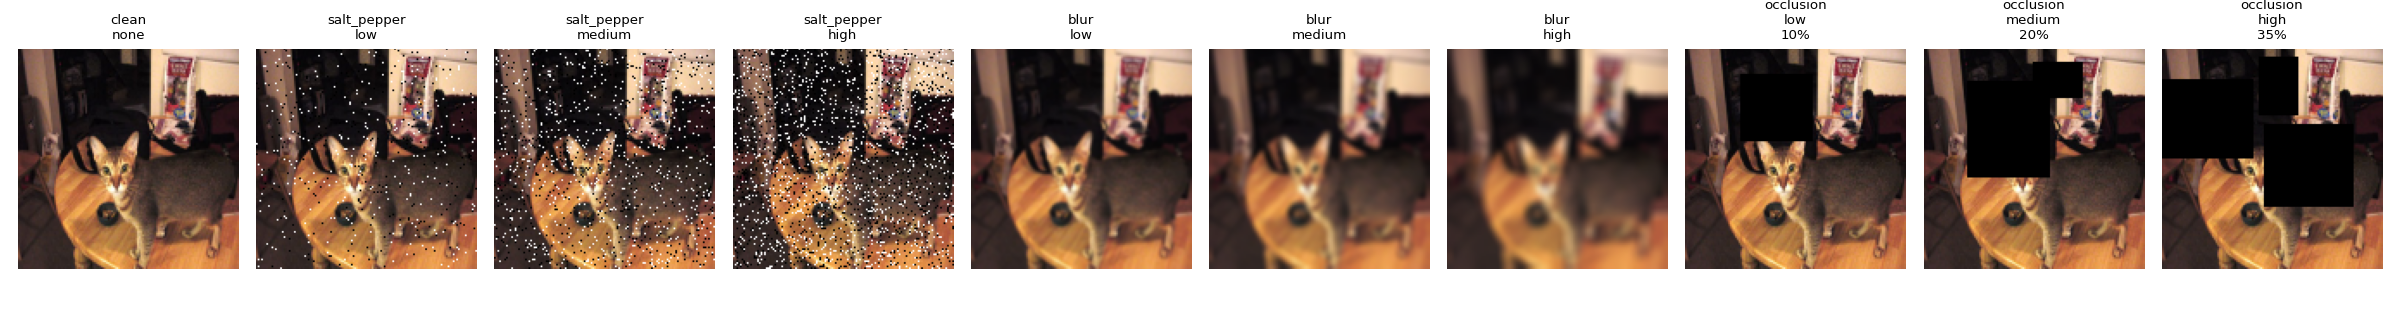
\includegraphics[width=\textwidth]{sanity_grid.png}
\caption{Corruption sanity grid produced by the shared corruption module (clean, salt-and-pepper, blur and
occlusion at several settings). It was inspected before training to confirm value ranges and that occlusion masks
respect the union-area limits.}\label{fig:sanity}
\end{figure*}

\textbf{FS2K}~\cite{fan2022}. We use the official split: 1,058 training and 1,046 test pairs. A stratified 15\%
validation split (seed 42) gives 899 training and 159 validation pairs (styles 1/2/3: 303/298/298 train,
54/52/53 val). A pairing script verified all 2,104 photo--sketch pairs (0 problems); RGBA and grayscale files are
converted to RGB. Augmentation is a random horizontal flip and a random resized crop (resize to $136$, crop $128$)
whose parameters are drawn once and applied to \emph{both} photo and sketch, preserving pixel correspondence.

% =====================================================================================================
\section{Experimental Setup}\label{sec:setup}
\textbf{Hardware and training.} All models were trained on an NVIDIA RTX~4050 Laptop GPU (6\,GB) with PyTorch~2.11
and bfloat16 autocast. Autoencoders, classifier and MoE use AdamW~\cite{loshchilov2019} with a cosine schedule
(with 100 linear warm-up steps for the autoencoders and the classifier, and gradient clipping at norm 1 for the
MoE); the GAN uses Adam~\cite{kingma2015} ($\beta_1=0.5$) with a constant learning rate for half of the
epochs followed by linear decay, as in pix2pix. Two engineering choices were measured before the long runs:
\texttt{cudnn.benchmark} was disabled because its auto-tuning added about 70\,s per run without a steady-state
speed-up, and data loading runs in the main process because Windows worker processes each re-import CUDA PyTorch
(1--4\,GB of committed memory), which exhausted the paging file and hung two parallel runs.

\textbf{Hyperparameter optimisation.} Every task uses an Optuna study with the TPE sampler (seed 42) and a
\texttt{MedianPruner} (3 start-up trials), stored in SQLite under \texttt{optuna\_studies/}. Trials are short
(4 epochs on a 50\% training subset for Tasks 1--2; 1 warm-up + 3 joint epochs for Task~3; 10 epochs for Task~4) and
the best configuration is then retrained for the full schedule. Table~\ref{tab:optuna} lists the search spaces and
the selected values. The restoration objective is
\begin{equation}
J = \tfrac12\,\min(\mathrm{PSNR},40)/40 + \tfrac12\,\mathrm{SSIM},\label{eq:obj}
\end{equation}
so both terms lie in $[0,1]$ and a perfect identity output (infinite PSNR) cannot dominate. The classifier is
selected by validation macro-F1, and the GAN by $\tfrac12(1-\ell_1)+\tfrac12\,\mathrm{SSIM}$ on the validation
sketches. The budget (10--15 trials) is small; this trade-off is discussed in Section~\ref{sec:limits}.

\begin{table}[!htbp]
\centering\caption{Optuna search spaces and selected values}\label{tab:optuna}
\scriptsize\setlength{\tabcolsep}{2.5pt}
\begin{tabular}{@{}lll@{}}
\toprule
Parameter & Range & Selected \\
\midrule
\multicolumn{3}{@{}l}{\textit{T1 universal DAE: 15 trials (10 complete, 5 pruned), best \#9, $J=0.468$}}\\
learning rate & $[3\!\cdot\!10^{-4}, 3\!\cdot\!10^{-3}]$ log & $4.61\cdot10^{-4}$\\
batch size & \{32, 64, 128\} & 32\\
latent channels (code $=c\times8\times8$) & \{8, 16, 32, 64\} & 8 (512 values)\\
encoder base channels & \{24, 32, 48\} & 48\\
dropout & $[0, 0.3]$ & 0.002\\
$\alpha$ ($\ell_1$ weight) & $[0.5, 0.95]$ & 0.730\\
\midrule
\multicolumn{3}{@{}l}{\textit{T2 classifier: 15 trials (8 complete, 7 pruned), best \#14, macro-F1 0.977}}\\
learning rate & $[3\!\cdot\!10^{-4}, 3\!\cdot\!10^{-3}]$ log & $1.00\cdot10^{-3}$\\
batch size & \{32, 64, 128\} & 32\\
channels & small/medium/wide & (32,64,128,256)\\
dropout & $[0, 0.5]$ & 0.249\\
weight decay & $[10^{-6}, 10^{-2}]$ log & $2.05\cdot10^{-4}$\\
\midrule
\multicolumn{3}{@{}l}{\textit{T2 specialists (shared search on blur): 12 trials (8/4), best \#9}}\\
same space as T1 & & same as T1 \\
\midrule
\multicolumn{3}{@{}l}{\textit{T3 soft MoE: 10 trials (9 complete, 1 pruned), best \#7, $J=0.865$}}\\
joint learning rate & $[10^{-5}, 3\!\cdot\!10^{-4}]$ log & $2.82\cdot10^{-5}$\\
temperature $\tau$ & $[0.5, 2.0]$ & 0.647\\
$\lambda_1$ ($\lambda_s=1-\lambda_1$) & $[0.5, 0.95]$ & 0.864\\
$\lambda_c$ (gate CE) & $[0.01, 0.5]$ log & 0.145\\
$\lambda_b$ (balance) & $[10^{-3}, 0.1]$ log & 0.0076\\
\midrule
\multicolumn{3}{@{}l}{\textit{T4 cGAN: 10 trials (8 complete, 2 pruned), best \#8, objective 0.687}}\\
G / D learning rate & $[5\!\cdot\!10^{-5}, 5\!\cdot\!10^{-4}]$ log & $3.21/3.94\cdot10^{-4}$\\
batch size & \{8, 16, 32\} & 8\\
generator base channels & \{32, 48, 64\} & 64\\
dropout & \{0, 0.25, 0.5\} & 0.25\\
style-embedding dim & \{8, 16, 32\} & 32\\
$\lambda_{L1}$ & $[10, 200]$ log & 168.6\\
\bottomrule
\end{tabular}
\end{table}

\textbf{Tracking.} Each final run logs hyperparameters, every loss term, validation metrics, sample grids from a
fixed validation batch and the best checkpoint (as a model artifact) to W\&B (\wandburl). The training curves in
this report are rebuilt from the local W\&B run files.

% =====================================================================================================
\section{Task 1: Universal Denoising Autoencoder}\label{sec:t1}
\begin{figure}[!htbp]
\centering
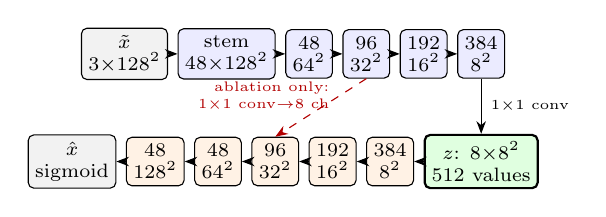
\begin{tikzpicture}[node distance=1.2mm]
\node[io] (x) {$\tilde{x}$\\3$\times$128$^2$};
\node[enc, right=of x] (e1) {stem\\48$\times$128$^2$};
\node[enc, right=of e1] (e2) {48\\64$^2$};
\node[enc, right=of e2] (e3) {96\\32$^2$};
\node[enc, right=of e3] (e4) {192\\16$^2$};
\node[enc, right=of e4] (e5) {384\\8$^2$};
\node[lat, below=7mm of e5] (z) {$z$: 8$\times$8$^2$\\512 values};
\node[dec, left=of z] (d1) {384\\8$^2$};
\node[dec, left=of d1] (d2) {192\\16$^2$};
\node[dec, left=of d2] (d3) {96\\32$^2$};
\node[dec, left=of d3] (d4) {48\\64$^2$};
\node[dec, left=of d4] (d5) {48\\128$^2$};
\node[io, left=of d5] (y) {$\hat{x}$\\sigmoid};
\foreach \a/\b in {x/e1,e1/e2,e2/e3,e3/e4,e4/e5,z/d1,d1/d2,d2/d3,d3/d4,d4/d5,d5/y} \draw[arr] (\a)--(\b);
\draw[arr] (e5)--node[right,font=\tiny]{1$\times$1 conv} (z);
\draw[arr, dashed, red!70!black] (e3.south) -- node[left,font=\tiny,align=right,pos=0.3]{ablation only:\\1$\times$1 conv$\to$8 ch} (d3.north);
\end{tikzpicture}
\caption{Task~1 denoising autoencoder (channels / spatial size). Encoder (blue) halves the resolution four times;
the latent code (green) is the only path to the decoder (orange). The dashed limited skip exists only in the
ablation of Section~\ref{sec:ablation}; the submitted model has no skip.}\label{fig:arch-ae}
\end{figure}

\begin{figure*}[t]
\centering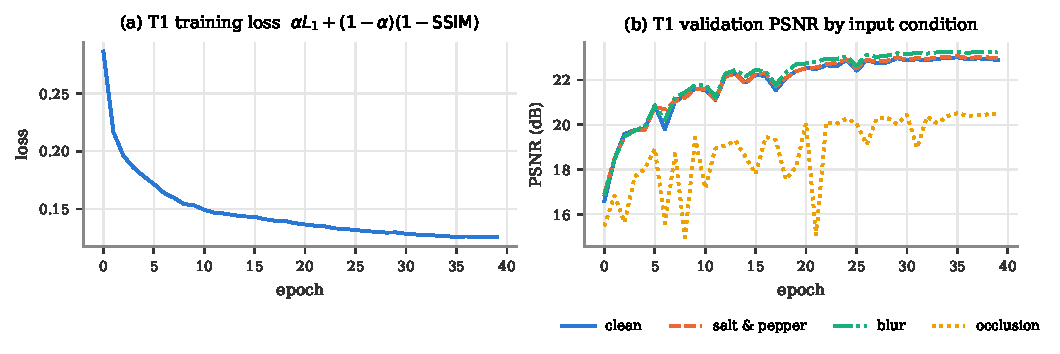
\includegraphics[width=\textwidth]{curves_t1.pdf}
\caption{Task~1 training loss and validation PSNR per input condition (validation manifest, 736 images).}
\label{fig:curves-t1}
\end{figure*}

\begin{figure*}[t]
\centering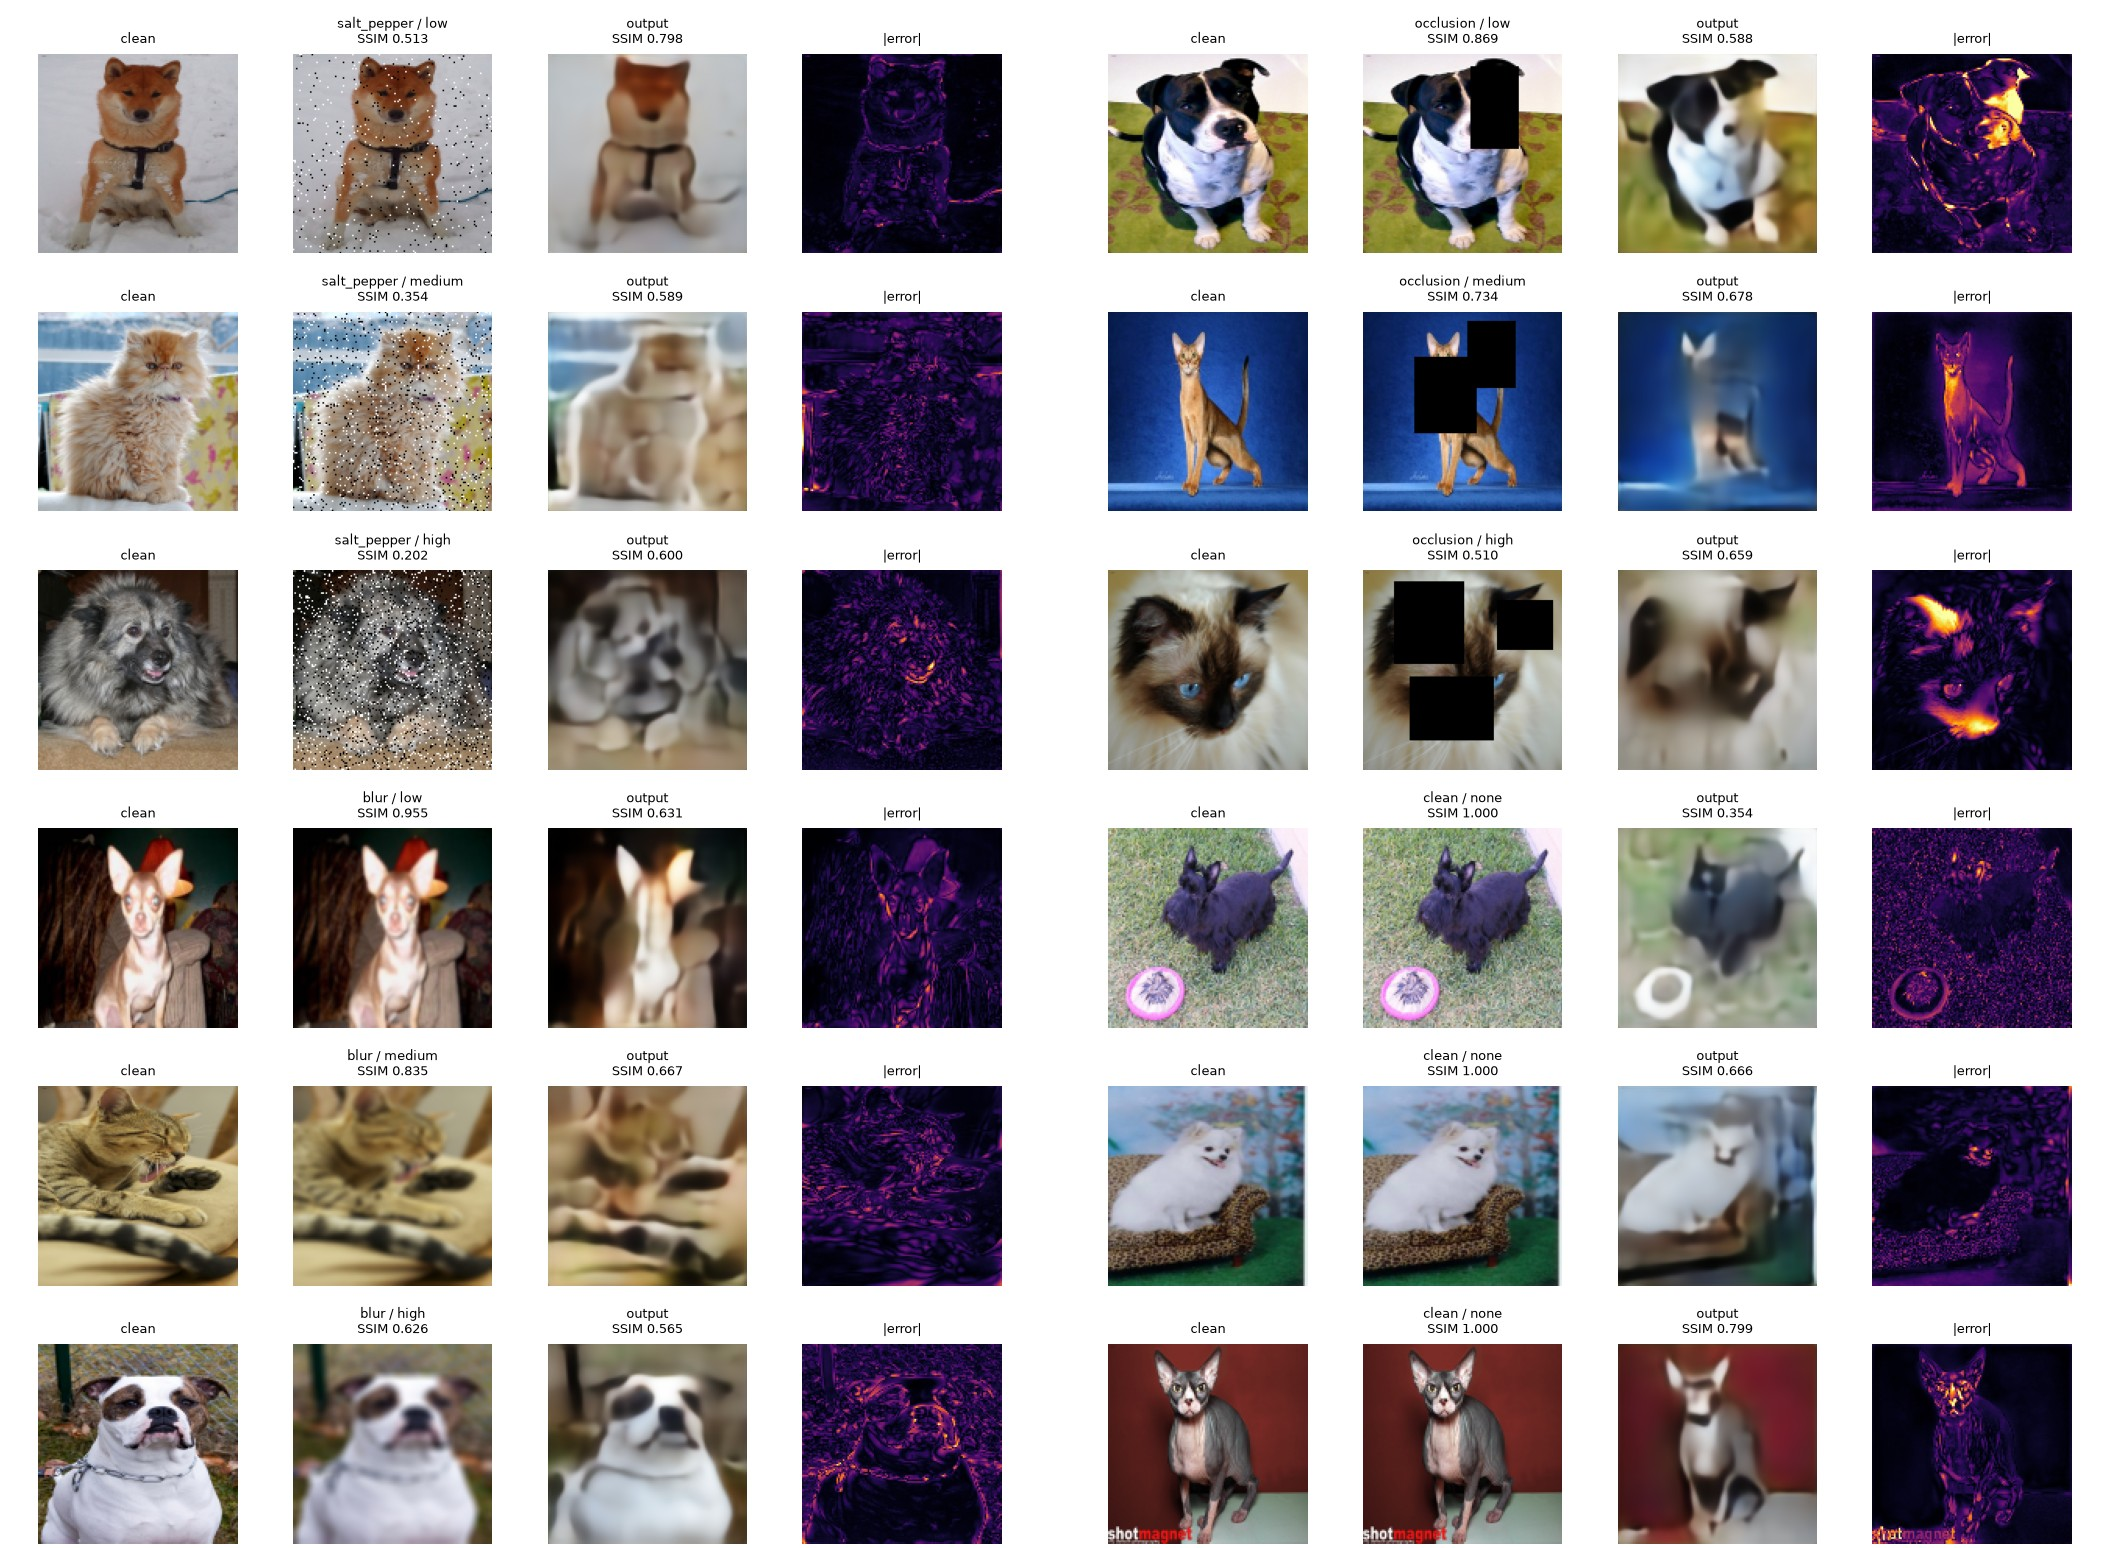
\includegraphics[width=0.86\textwidth]{t1_examples.jpg}
\caption{Task~1: twelve test examples (one per corruption and severity plus three clean images). Columns per example:
clean target, corrupted input, reconstruction, absolute error map (bright = large error).}\label{fig:t1-examples}
\end{figure*}

\begin{figure}[!htbp]
\centering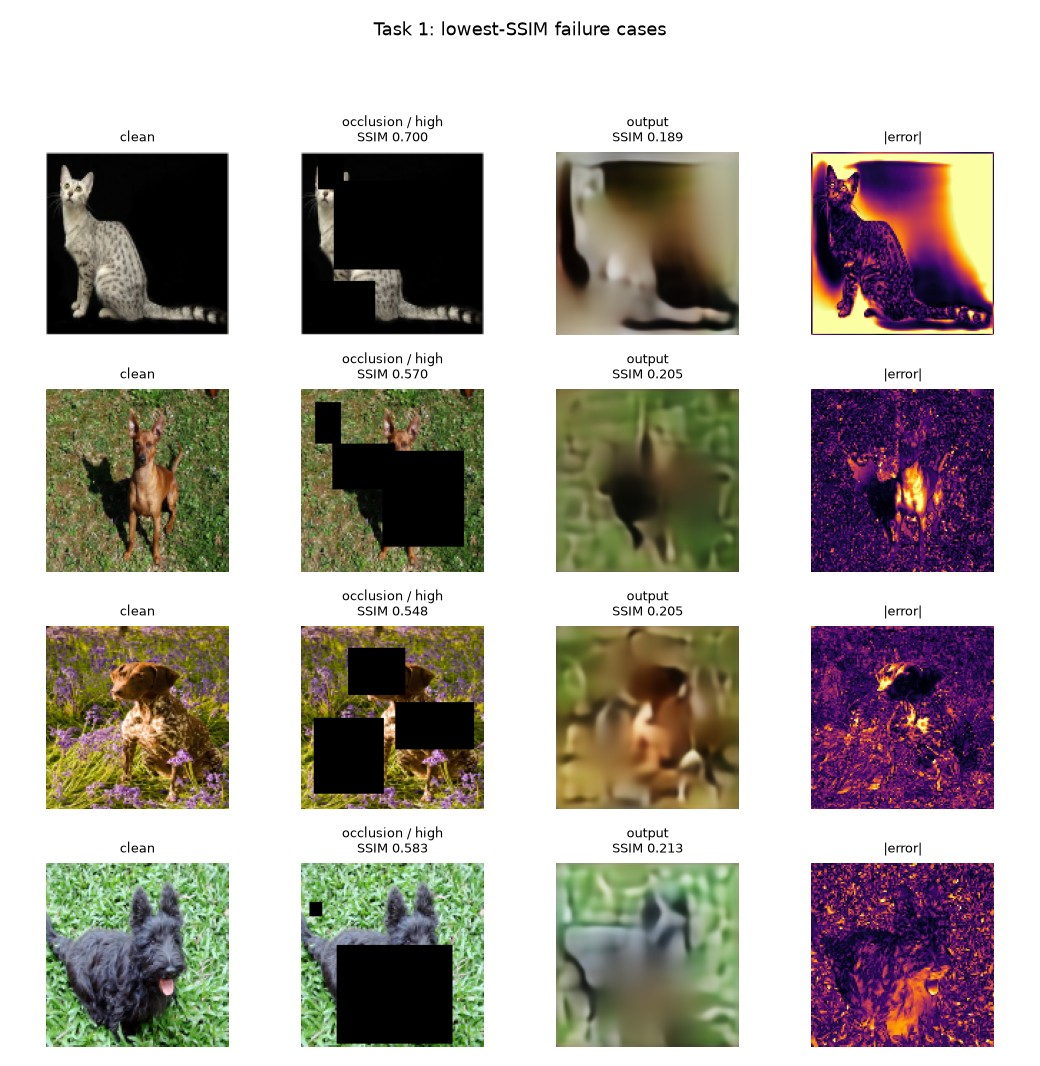
\includegraphics[width=\columnwidth]{t1_failures.jpg}
\caption{Task~1 failure cases (lowest output SSIM, distinct images).}\label{fig:t1-fail}
\end{figure}

\begin{figure}[!htbp]
\centering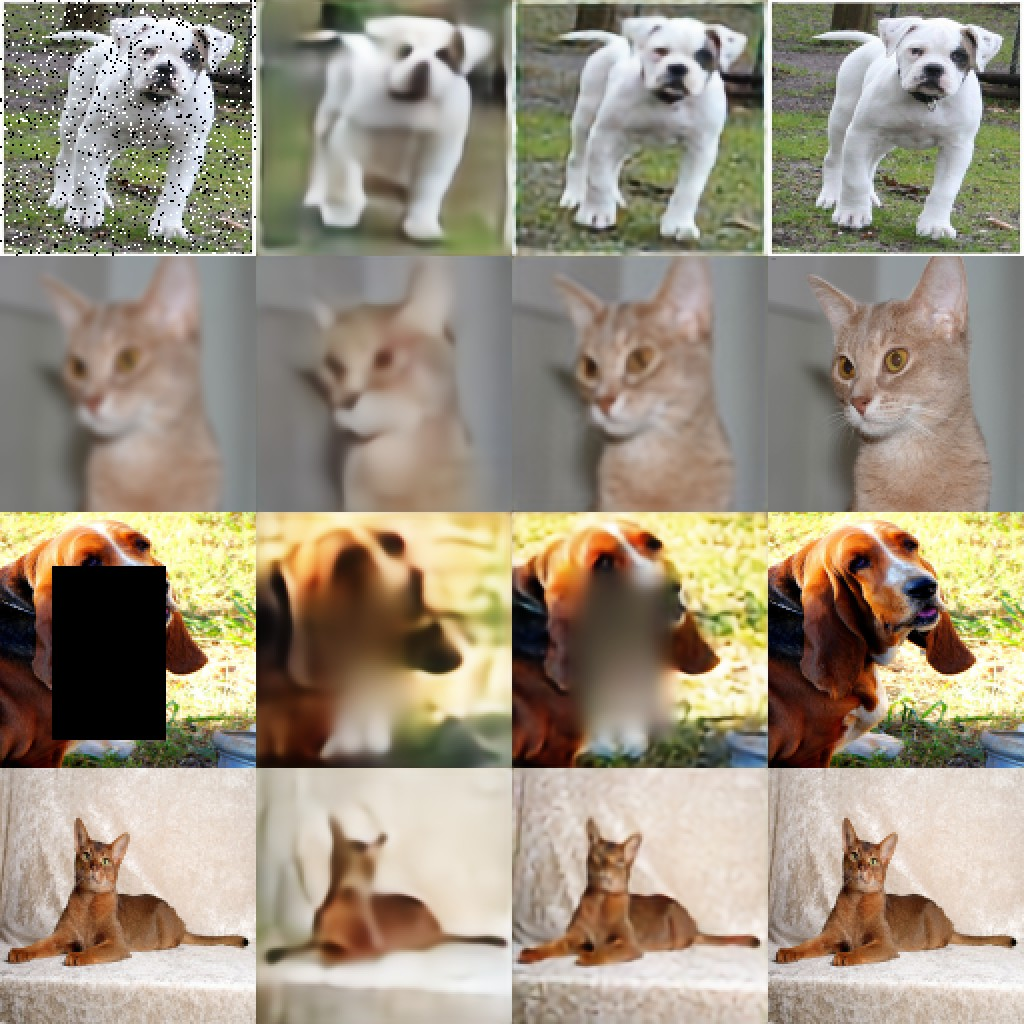
\includegraphics[width=0.8\columnwidth]{ablation_skip.jpg}
\caption{Ablation on validation images. Columns: corrupted input, selected model (no skip), model with one limited
skip, clean target. Rows: salt-and-pepper, blur, occlusion, clean.}\label{fig:ablation}
\end{figure}

\begin{figure}[!htbp]
\centering
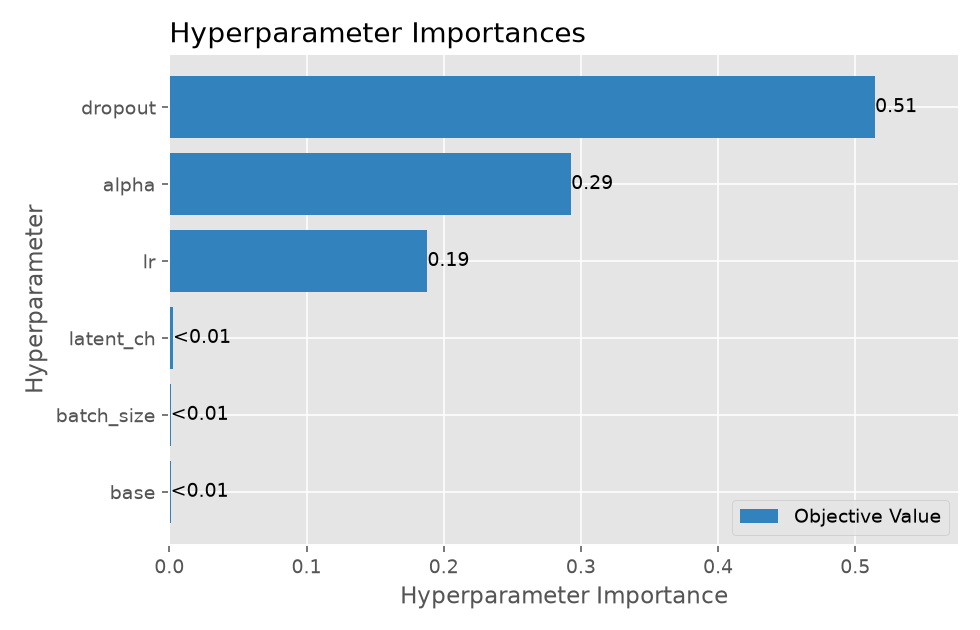
\includegraphics[width=0.49\columnwidth]{optuna_t1_importance.png}\hfill
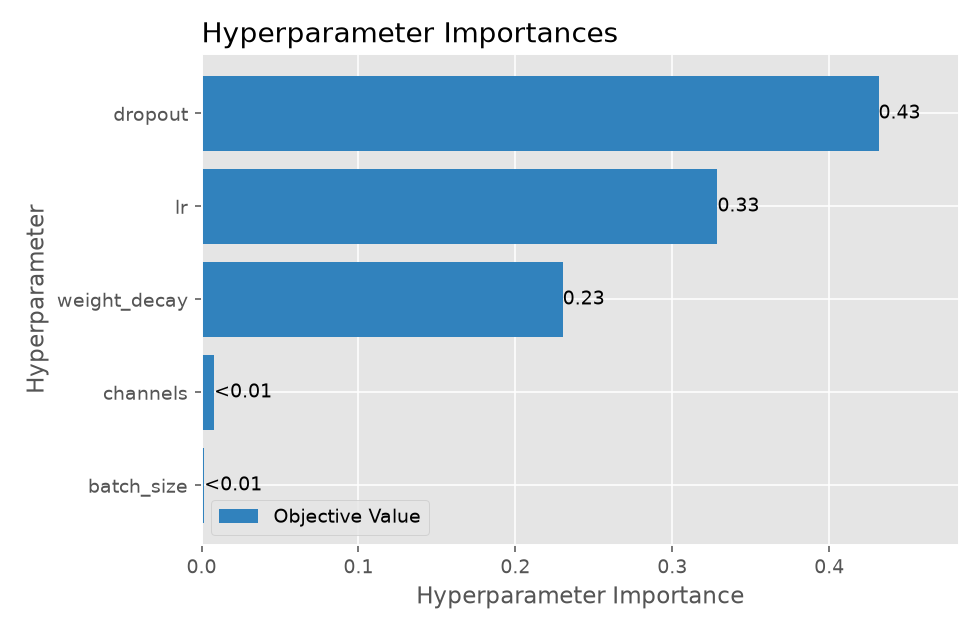
\includegraphics[width=0.49\columnwidth]{optuna_t2_cls_importance.png}\\[1mm]
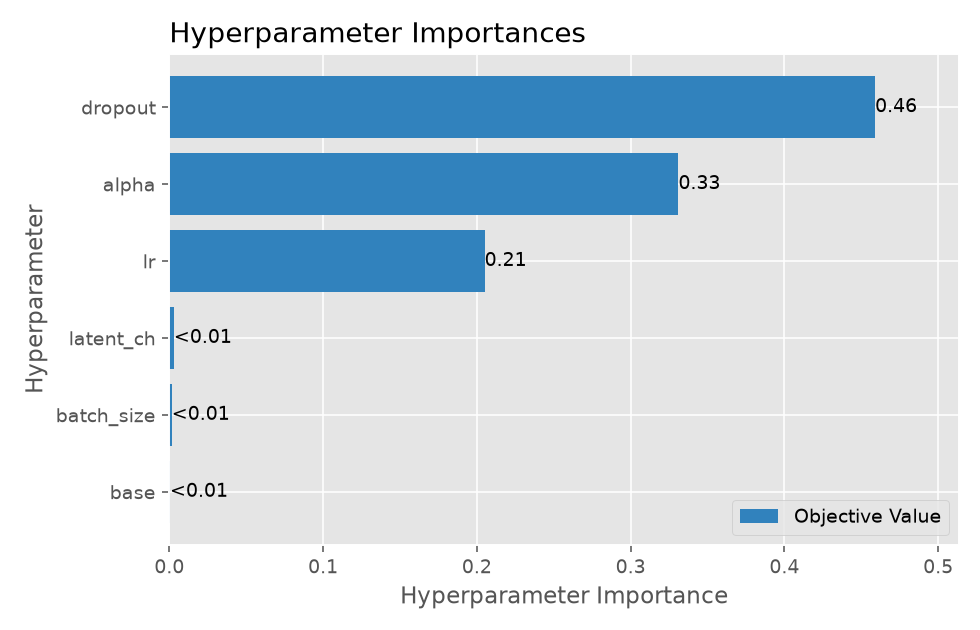
\includegraphics[width=0.49\columnwidth]{optuna_t2_spec_importance.png}\hfill
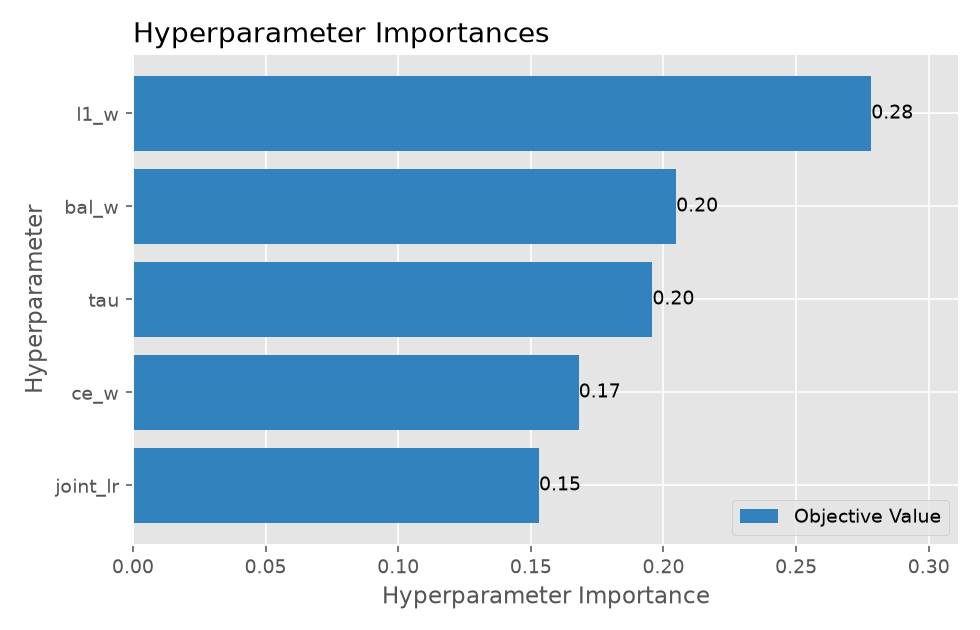
\includegraphics[width=0.49\columnwidth]{optuna_t3_importance.png}\\[1mm]
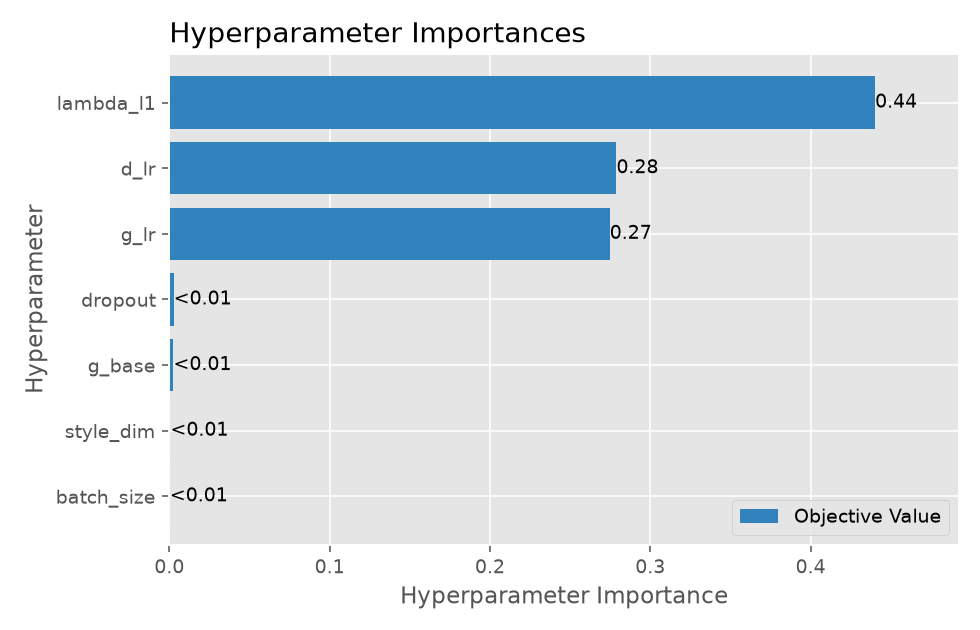
\includegraphics[width=0.49\columnwidth]{optuna_t4_importance.png}
\caption{Optuna hyperparameter importance (fANOVA) of the five studies: Task~1 DAE, classifier, shared specialist
search, soft MoE and cGAN (left to right, top to bottom). Optimisation histories are in \texttt{results/*/optuna/}.}
\label{fig:optuna-all}
\end{figure}

\textbf{Architecture} (Fig.~\ref{fig:arch-ae}). A stem and four stride-2 stages reduce $128\to8$ pixels while
widening channels to $b\cdot(1,2,4,8)$ with $b=48$; each stage has two $3\times3$ convolutions with batch norm and
GELU. A $1\times1$ convolution maps to the latent code of $c$ channels at $8\times8$. The decoder mirrors the encoder
with bilinear upsampling followed by convolutions, which avoids the checkerboard artefacts of transposed
convolutions~\cite{odena2016}, and ends with a sigmoid. With the selected $c=8$ the code holds 512 values for a
49,152-value input (96$\times$ compression), so the model cannot copy its input. It has 5.39\,M parameters. The loss
is $\mathcal{L}=\alpha\,\ell_1+(1-\alpha)(1-\mathrm{SSIM})$ with $\alpha=0.730$ chosen by Optuna (the brief
suggests 0.8 as a starting point).

\textbf{Training.} The selected configuration was trained for 40 epochs (22\,min). Fig.~\ref{fig:curves-t1} shows a
smoothly decreasing training loss. Validation PSNR rises for clean, salt-and-pepper and blurred inputs together and
levels off near 23\,dB after about 25 epochs, while occluded inputs stay about 2.5\,dB lower and fluctuate more,
because inventing the content behind a mask is the hardest of the four problems.

\textbf{Results.} Table~\ref{tab:t1} reports the untouched test set. The model removes salt-and-pepper noise
(+6.5\,dB, SSIM $0.38\to0.65$) and fills occlusions (+6.8\,dB), and the improvement grows with severity because the
corrupted input becomes worse while the output stays near 23\,dB. For blurred and clean inputs the output is
\emph{worse} than the input: the output quality is almost the same for every input (22.9--23.0\,dB), which is the
signature of an information bottleneck. Fine textures that survive mild blur do not fit through a 512-value code,
so the network returns a smooth reconstruction of the main shapes (Fig.~\ref{fig:t1-examples}). The error maps
concentrate on fur texture, edges and, for occlusions, the masked region.

\begin{table}[!htbp]
\centering\caption{Task~1 test results (PSNR in dB / SSIM). Clean input is identical to the target.}\label{tab:t1}
\scriptsize\setlength{\tabcolsep}{4pt}
\begin{tabular}{@{}llcccc@{}}
\toprule
Condition & Severity & PSNR in & PSNR out & SSIM in & SSIM out\\
\midrule
Clean & --- & $\infty$ & 22.89 & 1.000 & 0.653\\
\midrule
\multirow{3}{*}{Salt \& pepper} & low & 20.15 & 22.92 & 0.601 & 0.652\\
 & medium & 15.87 & 22.95 & 0.337 & 0.651\\
 & high & 13.14 & 22.92 & 0.201 & 0.647\\
\midrule
\multirow{3}{*}{Blur} & low & 32.15 & 22.99 & 0.937 & 0.654\\
 & medium & 26.89 & 23.12 & 0.804 & 0.649\\
 & high & 24.53 & 23.00 & 0.695 & 0.632\\
\midrule
\multirow{3}{*}{Occlusion} & low & 16.69 & 21.73 & 0.862 & 0.627\\
 & medium & 13.37 & 20.55 & 0.732 & 0.598\\
 & high & 10.80 & 18.98 & 0.549 & 0.550\\
\midrule
\multicolumn{2}{@{}l}{All 36,690 test items} & 27.36$^\ast$ & 22.20 & 0.672 & 0.631\\
\bottomrule
\multicolumn{6}{@{}l}{\tiny $^\ast$Includes clean inputs, whose PSNR is capped at 100\,dB.}
\end{tabular}
\end{table}

\textbf{Failure cases} (Fig.~\ref{fig:t1-fail}). The four lowest-SSIM test outputs (SSIM 0.19--0.21) are all
high-severity occlusions that hide most of the animal in front of a textured background (grass, flowers). The code
keeps the coarse layout, but the decoder fills the masks with a blurred average of the surrounding colours and also
smooths away the grass texture, so the error is spread over the whole image. It cannot hallucinate a head or fur
pattern, because $\ell_1$ and SSIM both reward the conditional mean rather than sharp but uncertain detail. The first
case is different: the photograph has a genuinely black background, and the model ``fills'' it like an occlusion,
which produces the bright error region --- the same black-region confusion that misleads the Task~2 classifier.

\subsection{Ablations: bottleneck size and one limited skip}\label{sec:ablation}
To find the cause of the 23\,dB ceiling we retrained Task~1 twice with everything else unchanged
(Table~\ref{tab:ablation}). Increasing the code from 8 to 64 channels (4,096 values) improves validation PSNR by only
0.8\,dB. Adding \emph{one} narrow skip --- the $32\times32$ encoder feature squeezed to 8 channels by a $1\times1$
convolution (8,192 values, still 6$\times$ smaller than the input) and joined to the decoder at the same resolution
--- raises PSNR by 4.9\,dB and SSIM from 0.64 to 0.84. Blur now ends above its input (28.8\,dB versus about 28\,dB)
instead of 5\,dB below it. The limit is therefore the $8\times8$ spatial resolution of the code, not its channel
count, which is consistent with the success of skip connections in restoration networks~\cite{mao2016}. Fig.~\ref{fig:ablation}
shows much sharper outputs; occlusion holes, however, are only blurred over, and a thin bright border appears on
salt-and-pepper inputs because noisy edge pixels leak through the skip. The submitted models keep
\texttt{skip=false} to respect the "genuine bottleneck" requirement without exception; adopting the skip would
require retraining Tasks~1--3.

\begin{table}[!htbp]
\centering\caption{Task~1 ablations (validation, last of 40 epochs, PSNR dB)}\label{tab:ablation}
\scriptsize\setlength{\tabcolsep}{3pt}
\begin{tabular}{@{}lcccccc@{}}
\toprule
Model & $J$ best & PSNR & SSIM & S\&P & Blur & Occl.\\
\midrule
Selected (code 8 ch, no skip) & 0.600 & 22.39 & 0.639 & 22.96 & 23.22 & 20.48\\
Code 64 ch, no skip & 0.630 & 23.15 & 0.681 & 23.84 & 24.11 & 20.82\\
Code 8 ch + one limited skip & \textbf{0.763} & \textbf{27.28} & \textbf{0.844} & \textbf{28.89} & \textbf{28.83} & \textbf{22.13}\\
\bottomrule
\end{tabular}
\end{table}

\textbf{Optuna analysis} (Fig.~\ref{fig:optuna-all}, top left). In the 4-epoch trials, dropout explains most of the variance
of the objective (importance 0.51; any noticeable dropout slows early learning), followed by $\alpha$ (0.29) and the
learning rate (0.19). Code size, batch size and width had importance below 0.01: within four epochs they made no
measurable difference, so the study's choice of the smallest code was effectively arbitrary. The 40-epoch ablation
shows that the code size \emph{does} matter for a full run (+0.8\,dB with 64 channels), i.e.\ short trials hid an
effect that appears only later in training. A longer trial budget or a multi-fidelity schedule would reduce this
bias.

% =====================================================================================================
\clearpage
\section{Task 2: Classifier and Hard-Routed Specialists}\label{sec:t2}
\begin{figure*}[t]
\centering
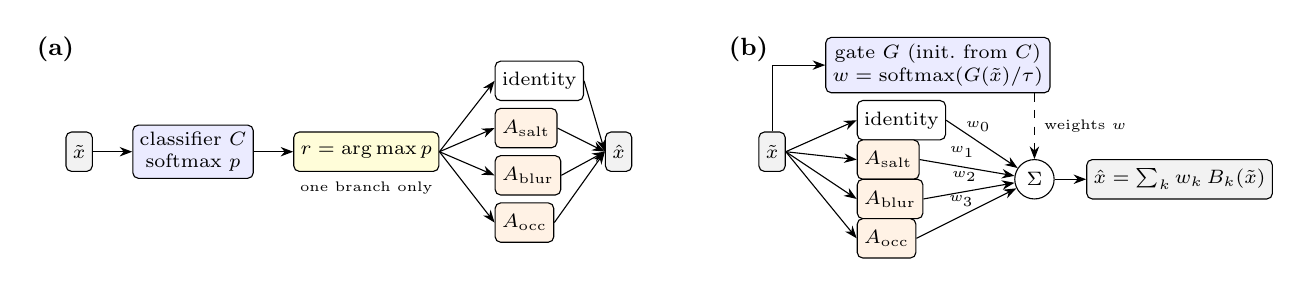
\begin{tikzpicture}[node distance=2mm]
% (a) hard routing
\node[font=\small\bfseries] at (-0.3,1.3) {(a)};
\node[io] (x) at (0,0) {$\tilde{x}$};
\node[enc, right=5mm of x] (c) {classifier $C$\\softmax $p$};
\node[blk, right=5mm of c, fill=yellow!15] (sw) {$r=\arg\max p$};
\node[blk, right=7mm of sw, yshift=9mm] (b0) {identity};
\node[dec, right=7mm of sw, yshift=3mm] (b1) {$A_\text{salt}$};
\node[dec, right=7mm of sw, yshift=-3mm] (b2) {$A_\text{blur}$};
\node[dec, right=7mm of sw, yshift=-9mm] (b3) {$A_\text{occ}$};
\node[io, right=6mm of b1, yshift=-3mm] (y) {$\hat{x}$};
\draw[arr] (x)--(c); \draw[arr] (c)--(sw);
\foreach \b in {b0,b1,b2,b3} {\draw[arr] (sw.east)--(\b.west); \draw[arr] (\b.east)--(y.west);}
\node[font=\tiny, below=0mm of sw] {one branch only};
% (b) soft MoE
\begin{scope}[xshift=88mm]
\node[font=\small\bfseries] at (-0.3,1.3) {(b)};
\node[io] (x2) at (0,0) {$\tilde{x}$};
\node[enc, right=5mm of x2, yshift=11mm] (g) {gate $G$ (init.\ from $C$)\\$w=\mathrm{softmax}(G(\tilde{x})/\tau)$};
\node[blk, right=9mm of x2, yshift=4mm] (s0) {identity};
\node[dec, right=9mm of x2, yshift=-1mm] (s1) {$A_\text{salt}$};
\node[dec, right=9mm of x2, yshift=-6mm] (s2) {$A_\text{blur}$};
\node[dec, right=9mm of x2, yshift=-11mm] (s3) {$A_\text{occ}$};
\node[blk, circle, right=12mm of s1, yshift=-2.5mm, inner sep=1pt] (sum) {$\Sigma$};
\node[io, right=4mm of sum] (y2) {$\hat{x}=\sum_k w_k\,B_k(\tilde{x})$};
\draw[arr] (x2.north)|-(g.west);
\foreach \b/\w in {s0/w_0,s1/w_1,s2/w_2,s3/w_3} {\draw[arr] (x2.east)--(\b.west); \draw[arr] (\b.east)--node[font=\tiny,above,pos=0.45]{$\w$}(sum);}
\draw[arr, dashed] (sum.north |- g.south) -- node[font=\tiny,right]{weights $w$} (sum.north);
\draw[arr] (sum)--(y2);
\end{scope}
\end{tikzpicture}
\caption{(a) Task~2 hard routing: the classifier picks exactly one branch; clean inputs bypass restoration.
(b) Task~3 soft MoE: every branch runs and the gate's continuous weights blend the identity branch and the three
experts; the whole pipeline is differentiable and exported as one ONNX graph that outputs the image and the weights.}
\label{fig:arch-route}
\end{figure*}

\begin{figure*}[t]
\centering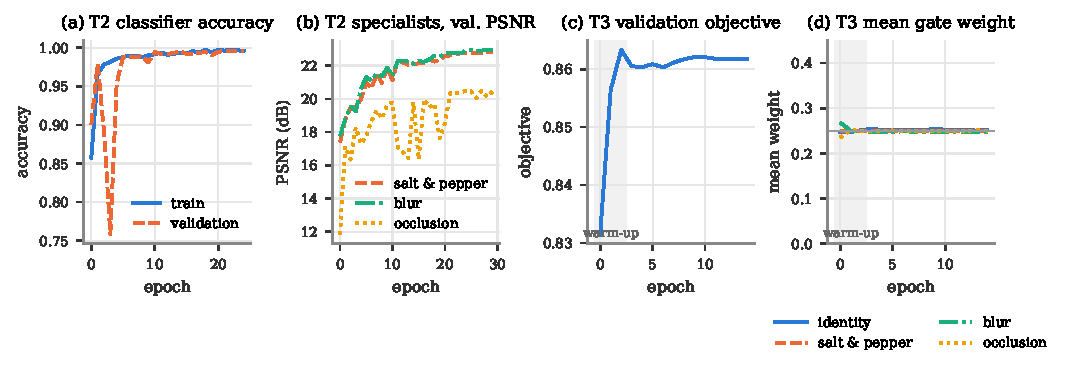
\includegraphics[width=\textwidth]{curves_t23.pdf}
\caption{Training curves of Tasks~2 and~3. (a) Classifier accuracy; validation shows one transient dip at epoch 3,
early in training when the learning rate is at its peak. (b) Validation PSNR of each specialist on its own corruption.
(c) MoE validation objective and (d) mean gate weight per branch; shaded epochs are the warm-up (experts frozen). The
weights stay at $\approx0.25$ each on the balanced validation set: no branch collapses or dies.}\label{fig:curves-t23}
\end{figure*}

\begin{figure}[!htbp]
\centering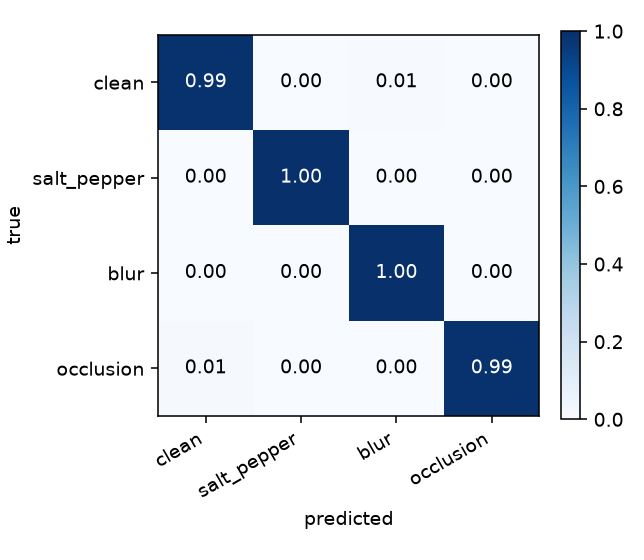
\includegraphics[width=0.62\columnwidth]{t2_confusion.png}
\caption{Normalised confusion matrix of the corruption classifier (rows: true class).}\label{fig:confusion}
\end{figure}

\begin{figure}[!htbp]
\centering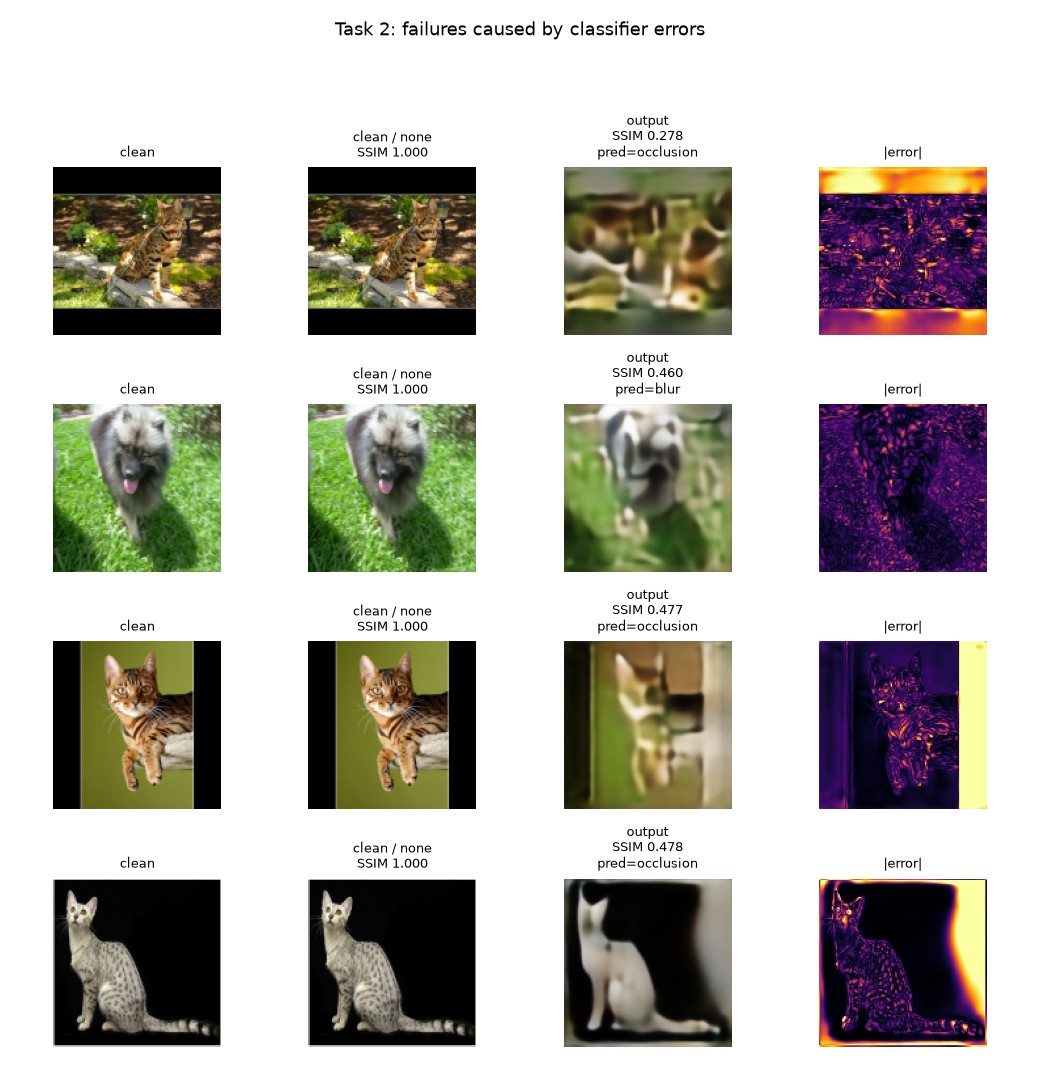
\includegraphics[width=\columnwidth]{t2_misrouting.jpg}
\caption{Task~2 failures caused by classifier errors: clean images with real black borders are classified as
occluded (``pred'') and blurred by the occlusion expert.}\label{fig:misroute}
\end{figure}

\textbf{Classifier.} Four convolutional stages (32--256 channels, two $3\times3$ conv + BN + ReLU each, then
$2\times2$ max pooling), global average pooling, dropout and a linear layer (1.17\,M parameters) predict
$p=[p_\text{clean},p_\text{salt},p_\text{blur},p_\text{occ}]$. It is trained with cross-entropy on balanced batches
for 25 epochs and selected by validation macro-F1.

\textbf{Specialists.} Three autoencoders with the Task~1 architecture are trained independently, each only on its own
corruption, for 30 epochs. A shared Optuna search (12 trials, run on the blur specialist as a proxy) chose the
architecture. Because the search space, sampler seed and the first 10 random start-up trials of TPE were identical to
Task~1, it selected the same configuration. Inference follows the brief: $r=\arg\max_k p_k$; clean images use the
identity bypass and are never processed by an expert (Fig.~\ref{fig:arch-route}a).

\textbf{Classifier results.} The test accuracy is 99.59\% with macro precision / recall / F1 of 0.991 / 0.995 /
0.993 (Table~\ref{tab:cls}, Fig.~\ref{fig:confusion}). Salt-and-pepper and blur are recognised perfectly. The only
systematic confusion is between \emph{clean} and \emph{occlusion}: 117 low-severity occlusions are called clean and
30 clean images are called blur (23) or occlusion (7). Fig.~\ref{fig:curves-t23}a shows that validation accuracy
reaches 99\% within six epochs.

\begin{table}[!htbp]
\centering\caption{Task~2 classifier on the test manifest (36,690 items)}\label{tab:cls}
\scriptsize
\begin{tabular}{@{}lcccc@{}}
\toprule
Class & Precision & Recall & F1 & Support\\
\midrule
Clean & 0.969 & 0.992 & 0.980 & 3,669\\
Salt \& pepper & 1.000 & 1.000 & 1.000 & 11,007\\
Blur & 0.998 & 1.000 & 0.999 & 11,007\\
Occlusion & 0.999 & 0.989 & 0.994 & 11,007\\
\midrule
Macro average & 0.991 & 0.995 & 0.993 & accuracy 0.996\\
\bottomrule
\end{tabular}
\end{table}

\textbf{Oracle versus predicted routing.} Table~\ref{tab:compare} compares all restoration systems per condition. Oracle and
predicted routing are almost identical (they differ only for the 0.8\% of clean images and 3.2\% of low occlusions that
are misrouted), so the operational system is limited by the specialists, not by the classifier. Surprisingly, the
specialists are \emph{not} better than the universal model on their own corruption (e.g.\ blur 22.77 versus
23.04\,dB): they share the same 512-value bottleneck, which removes the potential advantage of specialisation. The
real gain of hard routing is the identity bypass: clean images are returned untouched (SSIM 1.0) instead of being
degraded to 22.9\,dB by the universal model.

\begin{table}[!htbp]
\centering\caption{Test PSNR (dB) / SSIM per condition for all restoration systems}\label{tab:compare}
\scriptsize\setlength{\tabcolsep}{2.4pt}
\begin{tabular}{@{}lccccc@{}}
\toprule
Condition & Input & T1 universal & T2 oracle & T2 predicted & T3 soft MoE\\
\midrule
Clean & $\infty$/1.000 & 22.89/0.653 & $\infty$/1.000 & 99.4$^\ast$/0.997 & 93.3$^\ast$/0.996\\
Salt \& pepper & 16.39/0.380 & \textbf{22.93}/0.650 & 22.66/0.652 & 22.66/0.652 & 22.66/0.652\\
Blur & \textbf{27.86}/\textbf{0.812} & 23.04/0.645 & 22.77/0.647 & 22.77/0.647 & 22.78/0.647\\
Occlusion & 13.62/\textbf{0.714} & 20.42/0.592 & 20.51/0.595 & 20.52/0.598 & \textbf{20.57}/0.605\\
\bottomrule
\multicolumn{6}{@{}l}{\tiny $^\ast$Mean over items whose MSE is capped at $10^{-10}$ (100\,dB) when the identity branch returns the input.}
\end{tabular}
\end{table}

\textbf{Misrouting failures} (Fig.~\ref{fig:misroute}). The four restorations hurt most by a classifier error are
all \emph{clean} photographs that contain genuine black regions --- letterbox bars or a black background. The
classifier has learned ``large black rectangle $\Rightarrow$ occlusion'', which is exactly the training signal, so
these images are sent to the occlusion expert, which blurs the whole image (SSIM drops from 1.0 to 0.28--0.48).
Conversely, small low-severity masks that hide little structure are called clean and pass unrestored. Both errors
come from the definition of the corruption rather than from under-training; a remedy is to add letterboxed clean
images to training or to let a soft gate hedge between branches, which Task~3 does.

% =====================================================================================================
\clearpage
\section{Task 3: Soft Mixture of Experts}\label{sec:t3}
\begin{figure}[!htbp]
\centering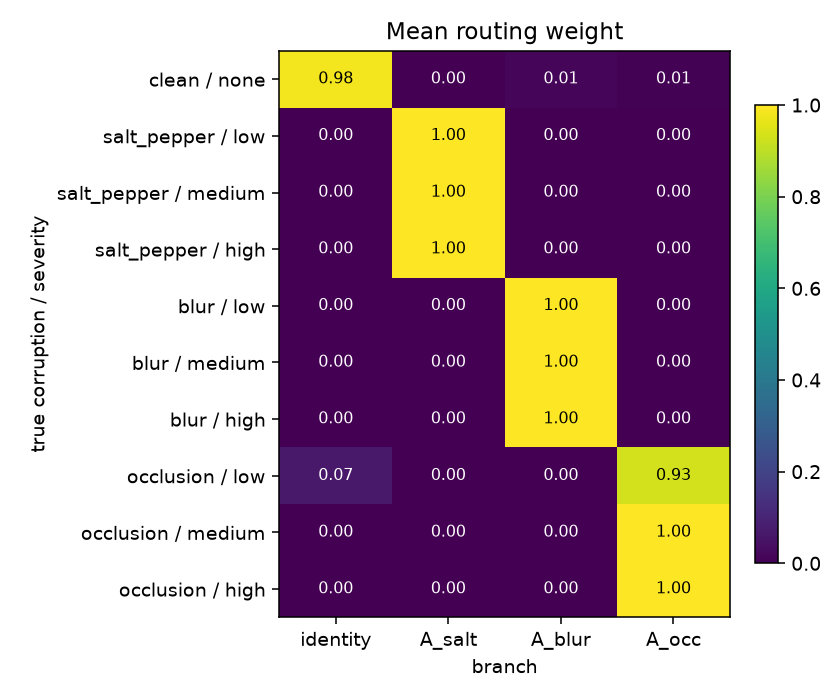
\includegraphics[width=0.78\columnwidth]{t3_heatmap.png}
\caption{Task~3 routing heatmap: mean gate weight per branch for every true corruption and severity (test set).}
\label{fig:heatmap}
\end{figure}

\begin{figure*}[t]
\centering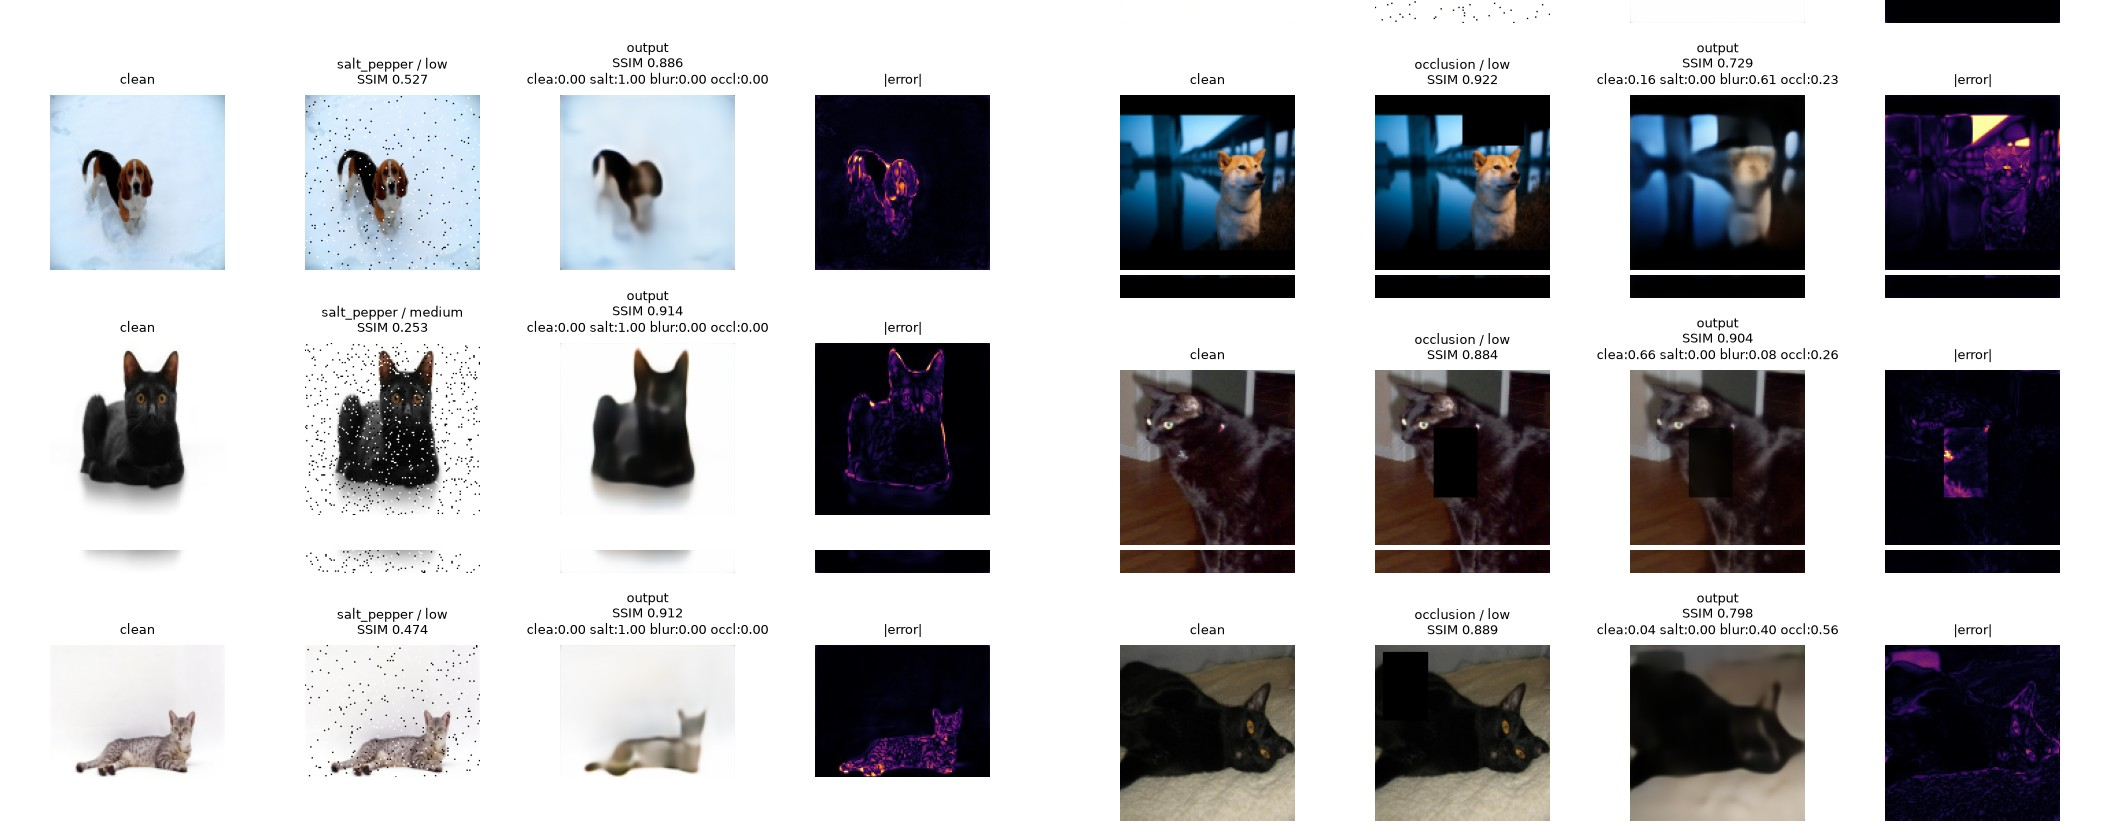
\includegraphics[width=\textwidth]{t3_dominant.jpg}
\caption{Task~3: dominant routing (left column: one expert receives weight 1.00) versus distributed routing (right
column: weights spread over several branches, shown above each output as clean/salt/blur/occlusion).}
\label{fig:dominant}
\end{figure*}

\textbf{Model.} The gate $G$ is a copy of the Task~2 classifier and the experts are copies of the three specialists,
plus an identity branch (Fig.~\ref{fig:arch-route}b): $w=\mathrm{softmax}(G(\tilde{x})/\tau)$ and
$\hat{x}=w_0\tilde{x}+w_1A_\text{salt}(\tilde{x})+w_2A_\text{blur}(\tilde{x})+w_3A_\text{occ}(\tilde{x})$
(17.3\,M parameters). Training starts with a 3-epoch warm-up in which the experts are frozen and only the gate learns
(learning rate $10^{-3}$), followed by 12 epochs of joint fine-tuning of all parameters with the smaller
Optuna-selected rate $2.8\cdot10^{-5}$. The loss is
\begin{equation}
\mathcal{L}=\lambda_1\ell_1+\lambda_s(1-\mathrm{SSIM})+\lambda_c\,\mathrm{CE}(G(\tilde{x}),y)+\lambda_b\sum_{k=0}^{3}\big(\bar{w}_k-\tfrac14\big)^2,
\end{equation}
where $\bar{w}_k$ is the mean weight of branch $k$ in a (balanced) batch. The balance term follows the auxiliary
losses of sparse MoEs~\cite{shazeer2017,fedus2022}; because every batch contains exactly one quarter of each
condition, its optimum coincides with correct routing, so it penalises collapse without fighting the CE term. Optuna
trials whose largest mean branch weight exceeded 0.9 on validation were treated as routing collapse and pruned.

\textbf{Training behaviour} (Fig.~\ref{fig:curves-t23}c,d). The validation objective rises during warm-up
($0.832\to0.856\to0.863$) and then stays flat between 0.860 and 0.862 for all 12 joint epochs. The checkpoint with the
best validation objective is therefore the \emph{end of warm-up}; in the delivered MoE the experts equal the Task~2
specialists and only the gate was trained. We kept this selection rule rather than overriding it, and also release the
final joint checkpoint. Joint fine-tuning cannot help much here: the experts are capped by their bottleneck
(Section~\ref{sec:ablation}) and a quarter of the objective comes from clean images, where the identity branch
already reaches the 40\,dB cap in~(\ref{eq:obj}).

\textbf{Routing analysis.} The gate assigns 99.3\% of test images to the correct branch. Fig.~\ref{fig:heatmap}
reports the mean weights for every true condition and severity: salt-and-pepper and blur receive a weight of 1.00 on
their expert at every severity; clean images give 0.98 to the identity branch; and low-severity occlusion is the only
cell with a noticeable split (0.93 occlusion expert, 0.07 identity), the same ambiguity that the classifier showed.
The share of images whose largest weight goes to each branch is 0.104 / 0.300 / 0.301 / 0.295 (identity / salt /
blur / occlusion), close to the manifest proportions 0.1 / 0.3 / 0.3 / 0.3, so no expert is inactive and none
dominates unrelated inputs.

Fig.~\ref{fig:dominant} contrasts dominant and distributed routing. The three lowest-entropy cases are
salt-and-pepper images routed with weight 1.00. The three highest-entropy cases are low-severity occlusions, e.g.\
weights (0.16, 0, 0.61, 0.23): the small mask makes the image look almost clean or slightly blurred, and the soft
gate hedges. Hedging is what Task~3 was designed for: on occlusion the MoE has the best SSIM of all systems
(0.605, Table~\ref{tab:compare}), and for low occlusions it improves SSIM from 0.636 (hard routing) to 0.657 because
uncertain images are no longer sent wholesale to the wrong branch. A weighted average of a sharp and a blurred
reconstruction can, however, also produce ghosting, as in the distributed example with weight 0.61 on the blur
expert.

% =====================================================================================================
\section{Task 4: Style-Conditioned Face-to-Sketch cGAN}\label{sec:t4}
\begin{figure}[!htbp]
\centering
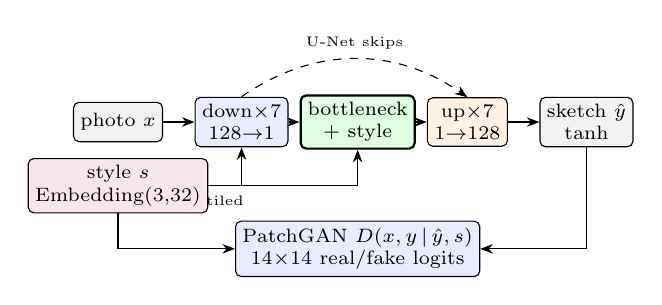
\begin{tikzpicture}[node distance=1.4mm]
\node[io] (x) {photo $x$};
\node[blk, below=2mm of x, fill=purple!10] (s) {style $s$\\Embedding(3,32)};
\node[enc, right=4mm of x] (d1) {down$\times$7\\128$\to$1};
\node[lat, right=of d1] (bn) {bottleneck\\+ style};
\node[dec, right=of bn] (u1) {up$\times$7\\1$\to$128};
\node[io, right=4mm of u1] (y) {sketch $\hat{y}$\\tanh};
\draw[arr] (x)--(d1); \draw[arr] (d1)--(bn); \draw[arr] (bn)--(u1); \draw[arr] (u1)--(y);
\draw[arr] (s.east)-|node[font=\tiny,below,pos=0.25]{tiled}(d1.south);
\draw[arr] (s.east)-|(bn.south);
\draw[arr, dashed] (d1.north) to[bend left=35] node[font=\tiny,above]{U-Net skips} (u1.north);
\node[enc, below=9mm of bn, minimum width=30mm] (D) {PatchGAN $D(x, y\,|\,\hat{y}, s)$\\14$\times$14 real/fake logits};
\draw[arr] (y.south)|-(D.east);
\draw[arr] (s.south)|-(D.west);
\end{tikzpicture}
\caption{Task~4 conditional GAN. The learned style embedding enters the generator at the input and at the bottleneck,
and the discriminator receives photo, (real or generated) sketch and the tiled embedding.}\label{fig:arch-gan}
\end{figure}

\begin{figure*}[t]
\centering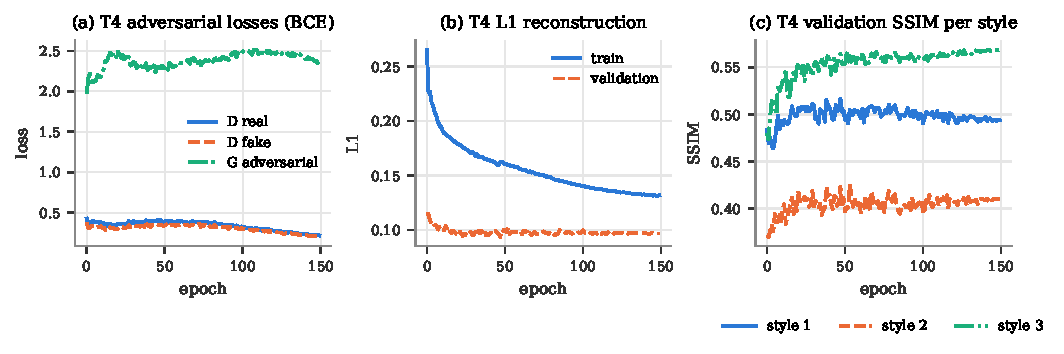
\includegraphics[width=\textwidth]{curves_t4.pdf}
\caption{Task~4 losses logged separately: discriminator real/fake and generator adversarial losses, generator $\ell_1$
on training versus validation, and validation SSIM per style.}\label{fig:curves-t4}
\end{figure*}

\begin{figure*}[t]
\centering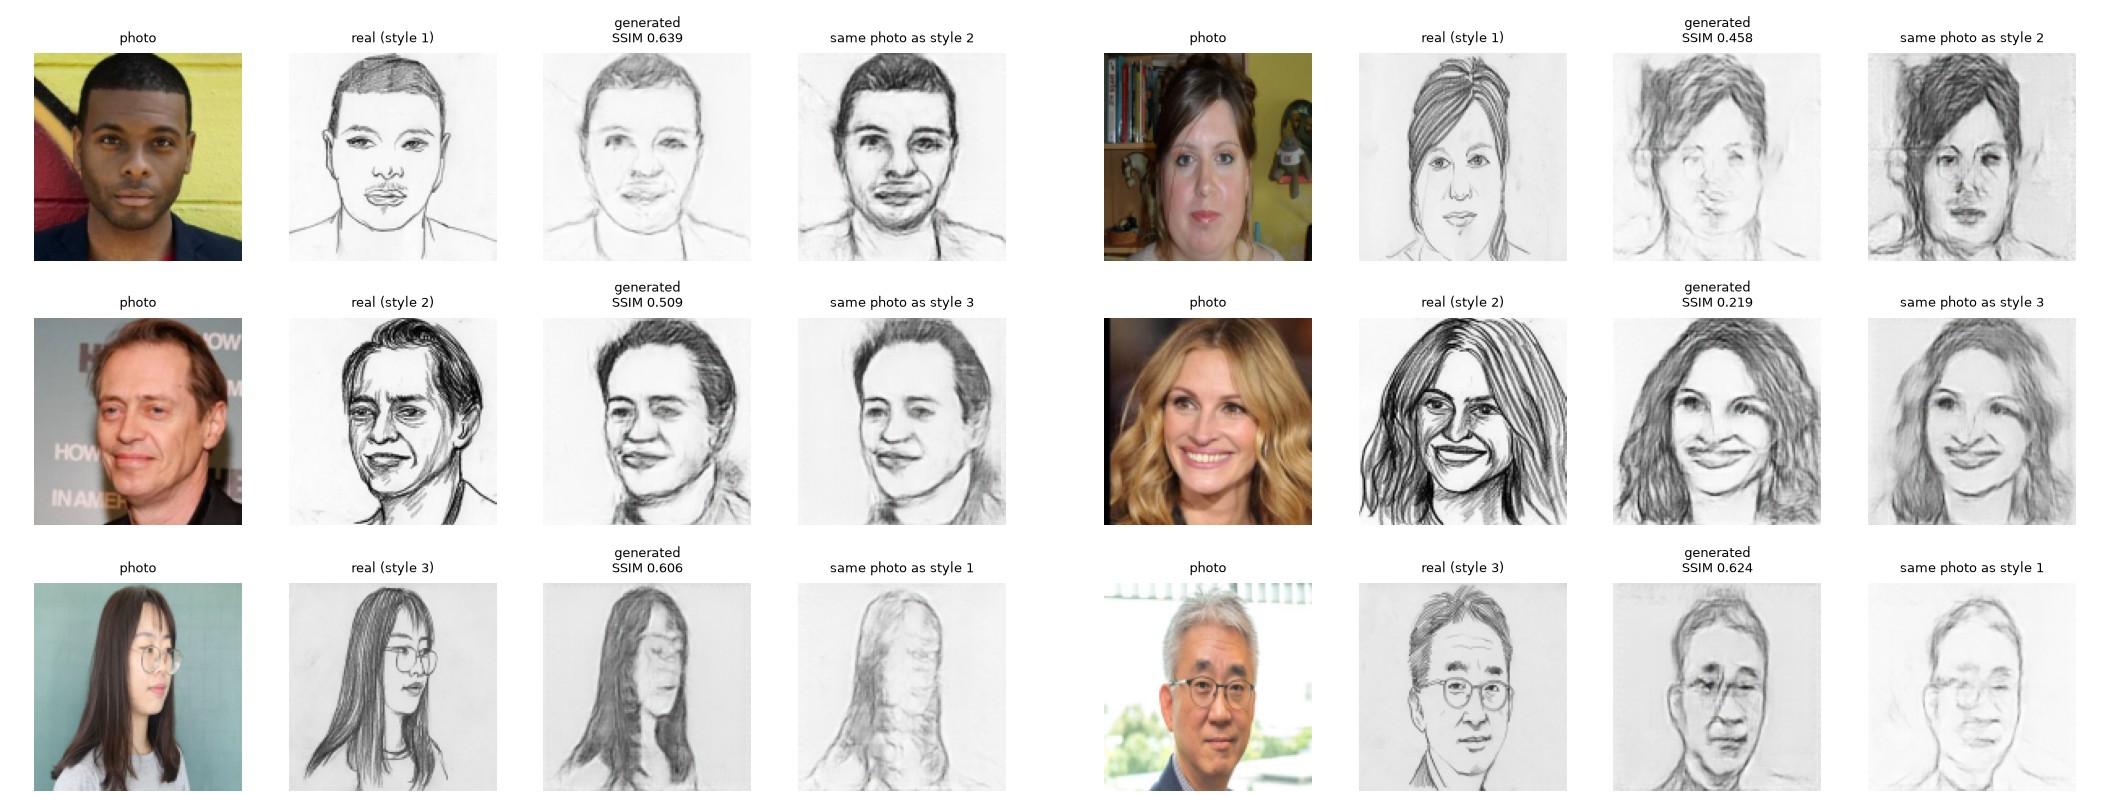
\includegraphics[width=\textwidth]{t4_examples.jpg}
\caption{Task~4 test examples, two per style (rows: style 1, 2, 3). Columns per example: photo, real sketch,
generated sketch in the true style, and the same photo generated in another style.}\label{fig:t4-examples}
\end{figure*}

\begin{figure}[!htbp]
\centering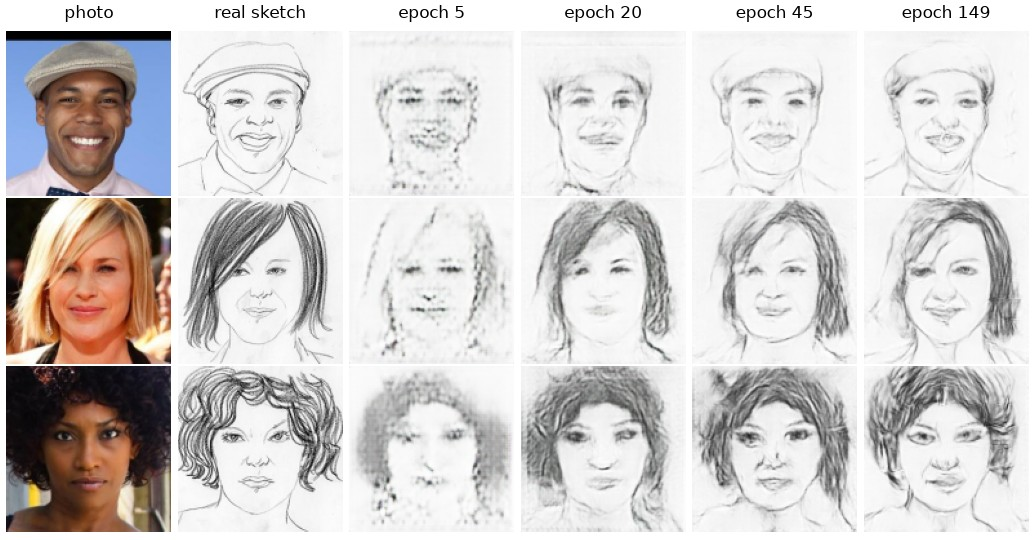
\includegraphics[width=\columnwidth]{t4_progress.jpg}
\caption{Task~4 generator development on fixed validation photographs (logged every 5 epochs; the selected
checkpoint is epoch 47).}\label{fig:t4-progress}
\end{figure}

\begin{figure}[!htbp]
\centering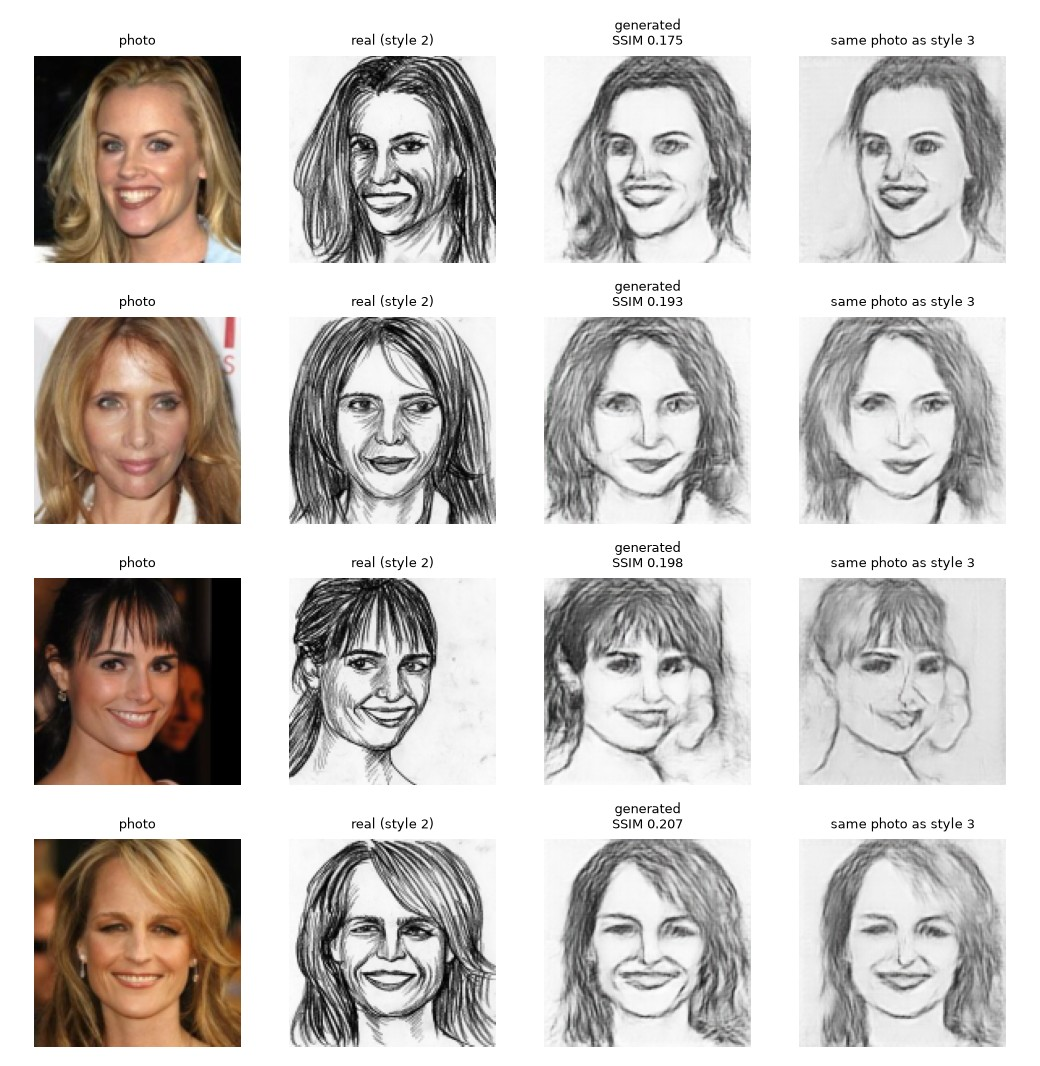
\includegraphics[width=\columnwidth]{t4_failures.jpg}
\caption{Task~4 failure cases (lowest SSIM): style-2 hatching on long hair.}\label{fig:t4-fail}
\end{figure}

\textbf{Architecture} (Fig.~\ref{fig:arch-gan}). The generator is a pix2pix U-Net~\cite{isola2017,ronneberger2015}
with seven stride-2 downsamplings ($128\to1$), instance normalisation~\cite{ulyanov2016}, dropout in the three
innermost decoder blocks and skip connections at every scale (42.1\,M parameters; skips are allowed here because
the input and output share structure). The style $s\in\{1,2,3\}$ is a learned \texttt{nn.Embedding}$(3,32)$ that is
injected twice into the generator --- tiled as 32 extra input channels and concatenated again at the $1\times1$
bottleneck --- and once into the discriminator. The discriminator is a PatchGAN (2.8\,M parameters) on the
concatenation of photo, sketch and tiled style embedding, producing $14\times14$ real/fake logits, i.e.\ it judges
whether each local patch is a plausible sketch \emph{of that style} for \emph{that photo}. Losses use binary
cross-entropy with logits: $\mathcal{L}_D=\mathrm{BCE}(D(x,y,s),1)+\mathrm{BCE}(D(x,G(x,s),s),0)$ and
$\mathcal{L}_G=\mathrm{BCE}(D(x,G(x,s),s),1)+\lambda_{L1}\,\lVert y-G(x,s)\rVert_1$ with $\lambda_{L1}=168.6$
selected by Optuna (pix2pix uses 100).

\textbf{Training} (Fig.~\ref{fig:curves-t4}). The selected configuration (batch 8) was trained for 150 epochs
(33\,min). The discriminator losses stay around 0.3--0.4 and decrease slowly as the learning rate decays, while the
generator's adversarial loss stays around 2.3--2.5: neither network wins, so training is stable. The training $\ell_1$
keeps falling, but the validation $\ell_1$ is flat after about 20 epochs and the best validation score occurs at
epoch 47; afterwards the generator mainly fits training-set stroke detail, which is expected with 899 training pairs.
The checkpoint selected on validation is therefore from epoch 47. Fig.~\ref{fig:t4-progress} follows three fixed validation photographs
through training: at epoch~5 the generator produces noisy, blotchy outlines; by epoch~20 the face contours and hair
masses are in place; around the selected epoch the strokes become clean and style-consistent. The final epoch draws
visibly sharper, more detailed strokes, yet its validation $\ell_1$ and SSIM are no better: the extra detail is not
where the artist put it, which is why the validation-based selection prefers epoch 47. Choosing the final model by a
pixel metric therefore trades some perceived sharpness for alignment, a known limitation of $\ell_1$/SSIM for
sketches.

\textbf{Results.} On the 1,046 official test pairs the generator reaches $\ell_1=0.103$ and SSIM 0.481
(Table~\ref{tab:t4}). Styles 1 and 3, which are line drawings and soft shaded sketches with large white areas, are
reproduced well (SSIM 0.52 and 0.61). Style~2, drawn with dense dark hatching, is the hardest (SSIM 0.40): even a
plausible sketch places its individual strokes differently from the artist, and pixel-aligned metrics punish every
misplaced stroke. Fig.~\ref{fig:t4-examples} shows that the embedding has a real effect: the same photograph rendered
as another style changes line weight and shading accordingly, so the condition is not ignored.

\begin{table}[!htbp]
\centering\caption{Task~4 test results per style (1,046 official test pairs)}\label{tab:t4}
\scriptsize
\begin{tabular}{@{}lcc@{}}
\toprule
Style & $\ell_1$ ($\downarrow$) & SSIM ($\uparrow$)\\
\midrule
Style 1 & 0.076 & 0.523\\
Style 2 & 0.152 & 0.397\\
Style 3 & 0.064 & 0.613\\
\midrule
All & 0.103 & 0.481\\
\bottomrule
\end{tabular}
\end{table}

\textbf{Failure cases} (Fig.~\ref{fig:t4-fail}). The lowest-SSIM outputs are all style-2 portraits with long hair. The
generated sketches are recognisable and in the right style, but hair strands and hatching do not align with the
reference, which yields SSIM below 0.21. Background clutter can also be drawn as strokes. A data issue also affects
the per-style numbers: the official test annotation labels 179 sketches from the \texttt{photo3} folder as style~1,
although the sketches we inspected resemble the pencil style labelled style~3 elsewhere. We kept the official labels
as required, and note that per-style test numbers may be slightly mixed.

\textbf{Optuna across tasks} (Fig.~\ref{fig:optuna-all}). For the classifier, dropout (0.43), learning rate (0.33)
and weight decay (0.23) explain almost all variance, while the channel configuration and batch size do not matter in
short trials. The specialist search repeats the Task~1 pattern (dropout, $\alpha$, learning rate). For the MoE the
importance is spread over all five parameters (reconstruction weight 0.28, balance weight and $\tau$ 0.20 each,
classification weight 0.17, joint learning rate 0.15): the gate, initialised from an accurate classifier, is already
close to optimal, so each parameter changes the objective only slightly. For the GAN, $\lambda_{L1}$ is the most
important parameter (0.44), followed by the two learning rates (0.28 and 0.27); style-embedding size, width, dropout
and batch size had little effect in 10-epoch trials, and the search moved $\lambda_{L1}$ above the usual
100~\cite{isola2017}.

% =====================================================================================================
\section{Application and Deployment}\label{sec:app}
\begin{figure*}[t]
\centering
\IfFileExists{figures/stitch_01_universal.png}{%
\includegraphics[width=0.245\textwidth]{stitch_01_universal.png}\hfill
\includegraphics[width=0.245\textwidth]{stitch_02_hard.png}\hfill
\includegraphics[width=0.245\textwidth]{stitch_03_moe.png}\hfill
\includegraphics[width=0.245\textwidth]{stitch_04_sketch.png}}{%
\fbox{\parbox{0.9\textwidth}{\centering\vspace{8mm}\TODO{Google Stitch design screenshots: save them as
docs/stitch/01\_universal.png, 02\_hard.png, 03\_moe.png, 04\_sketch.png and run
python -m scripts.report\_figures}\vspace{8mm}}}}
\caption{Original Google Stitch design of the four workspaces (evidence of the design step).}\label{fig:stitch}
\end{figure*}

\begin{figure*}[t]
\centering
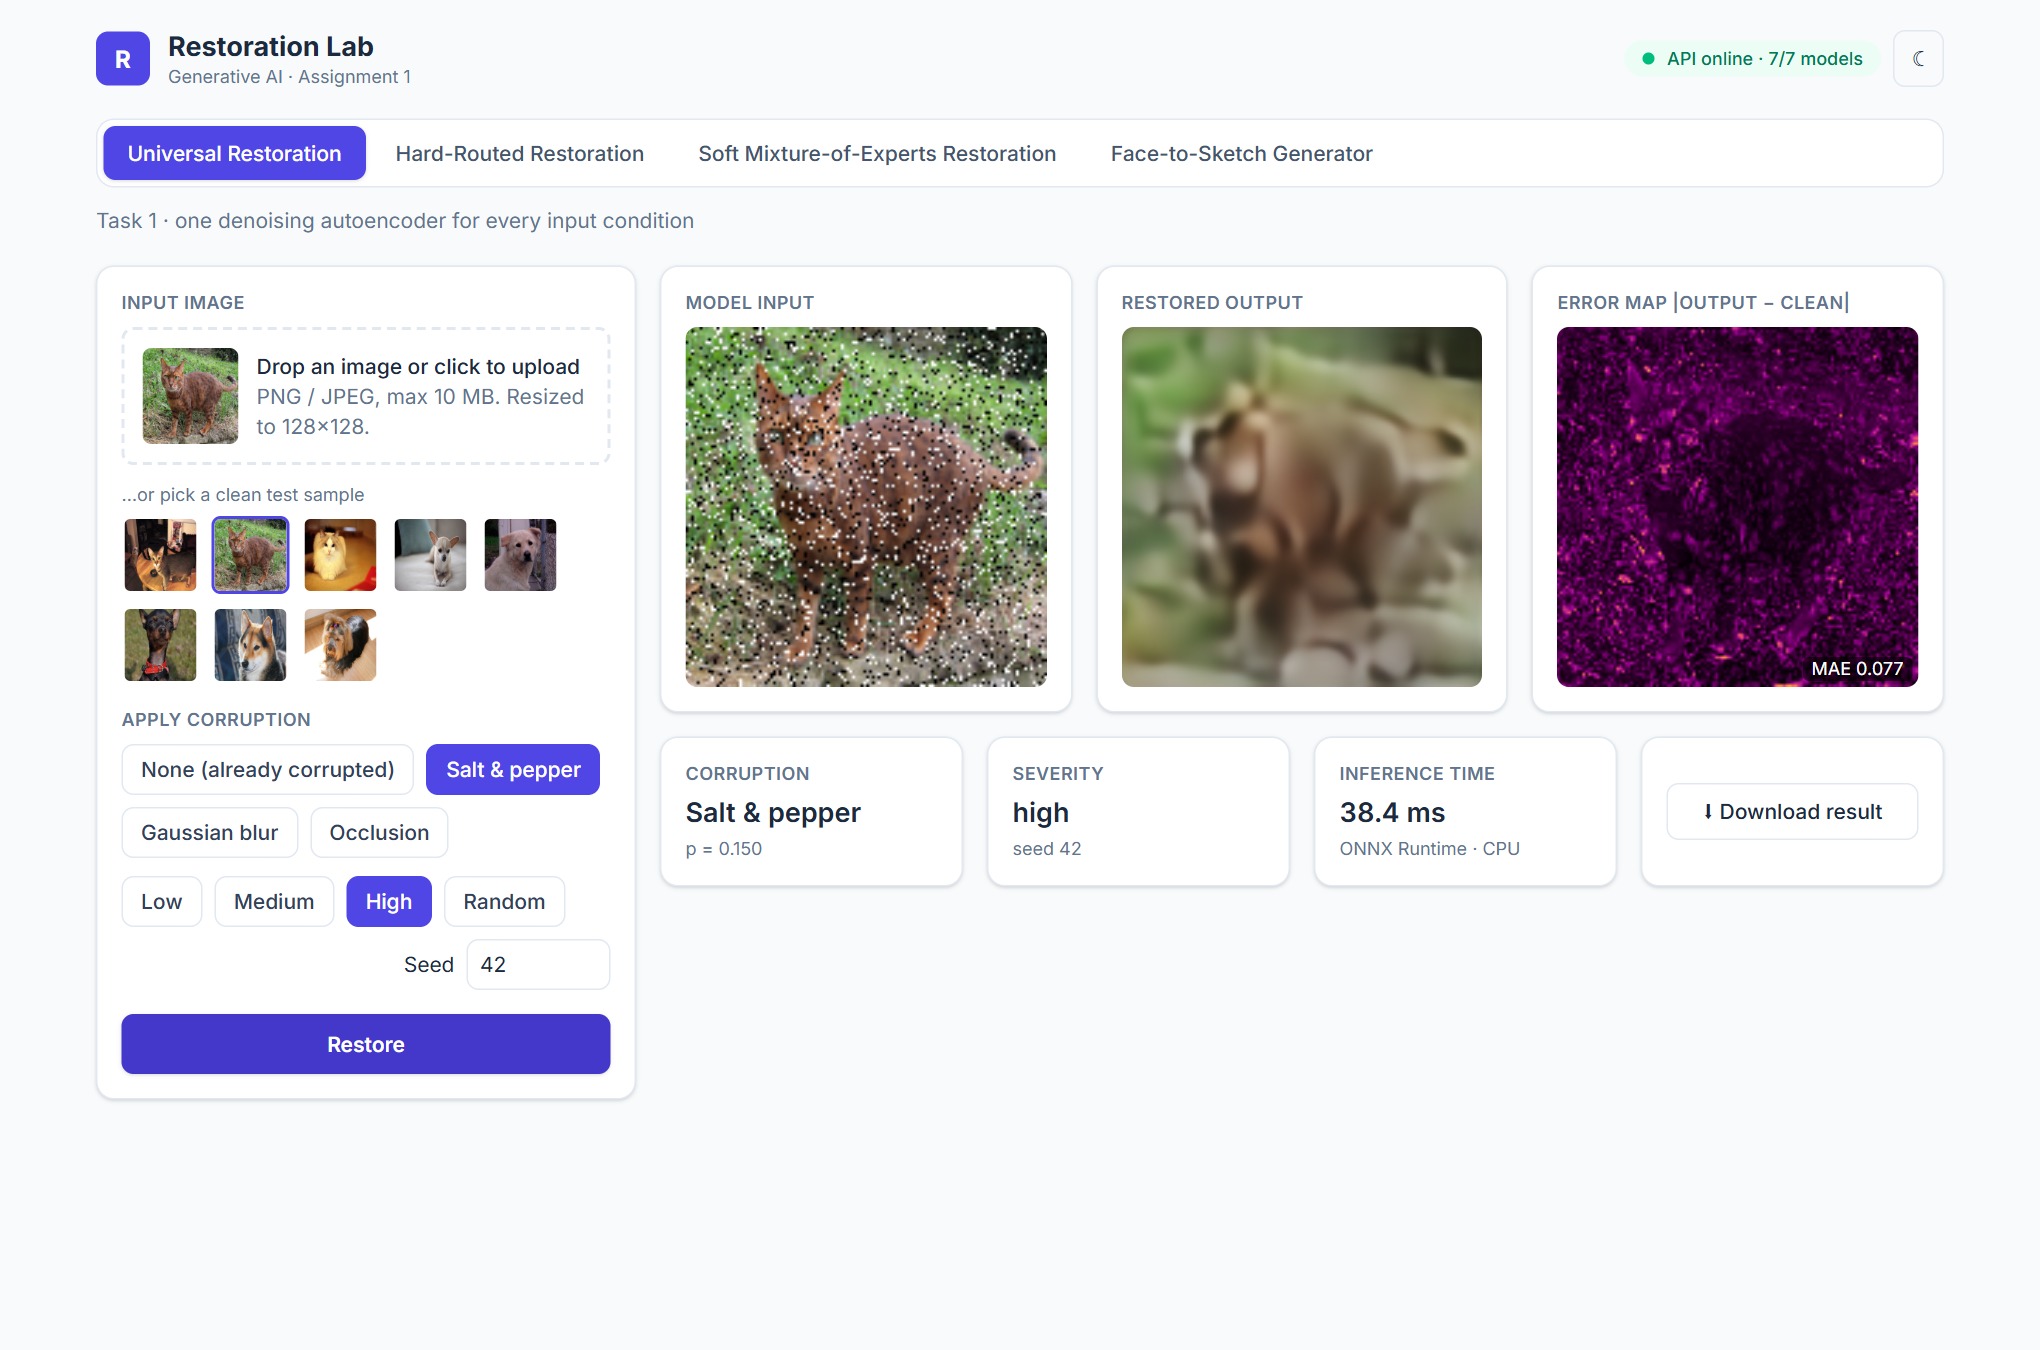
\includegraphics[width=0.42\textwidth]{app_universal.png}\hspace{2mm}
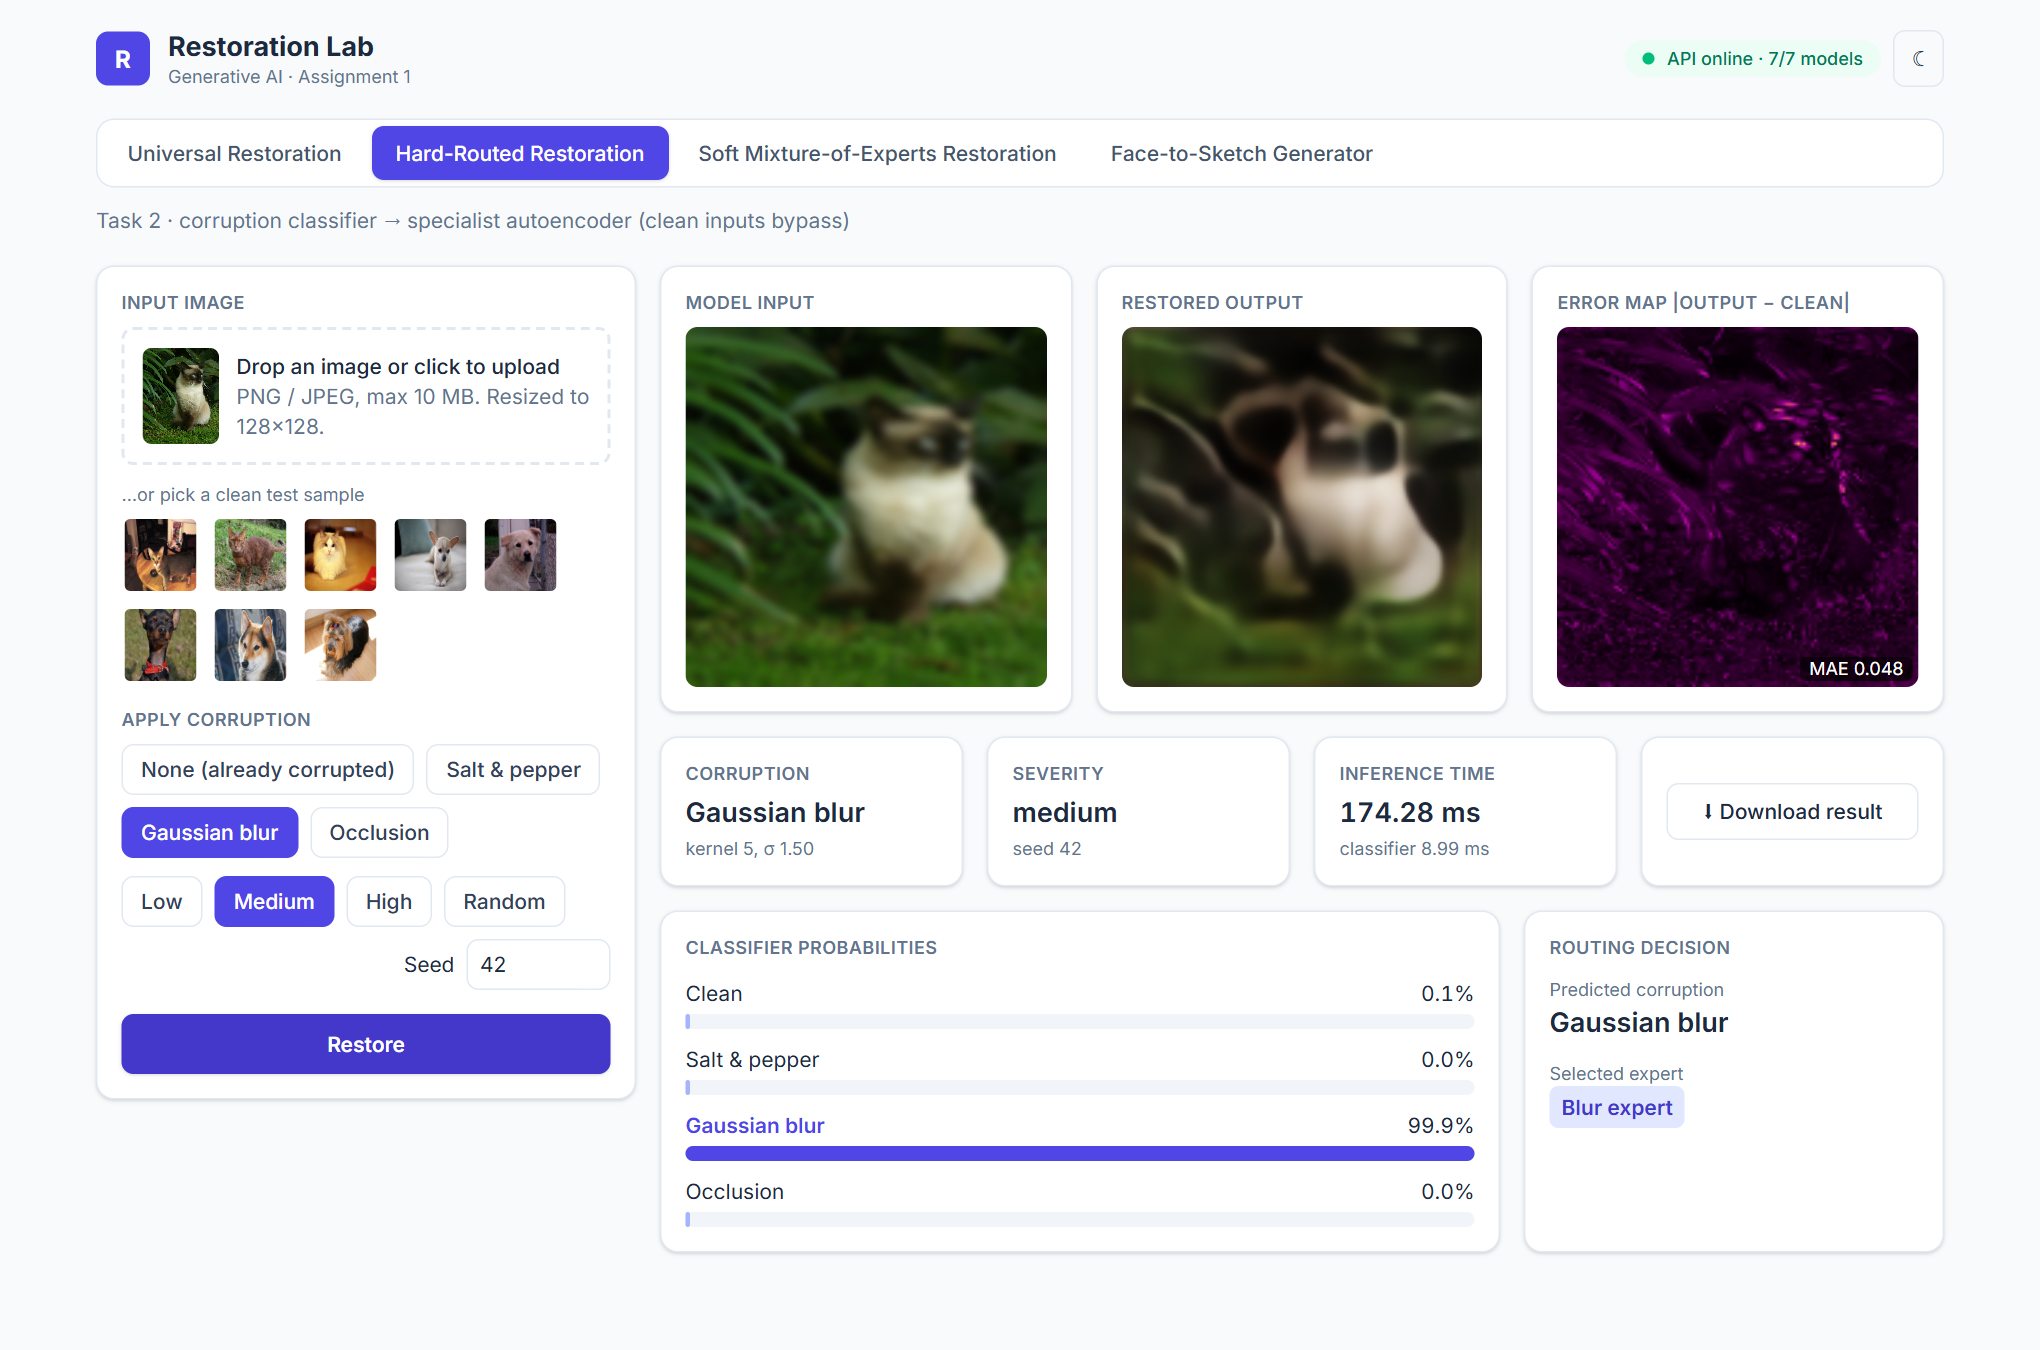
\includegraphics[width=0.42\textwidth]{app_hard.png}\\[1mm]
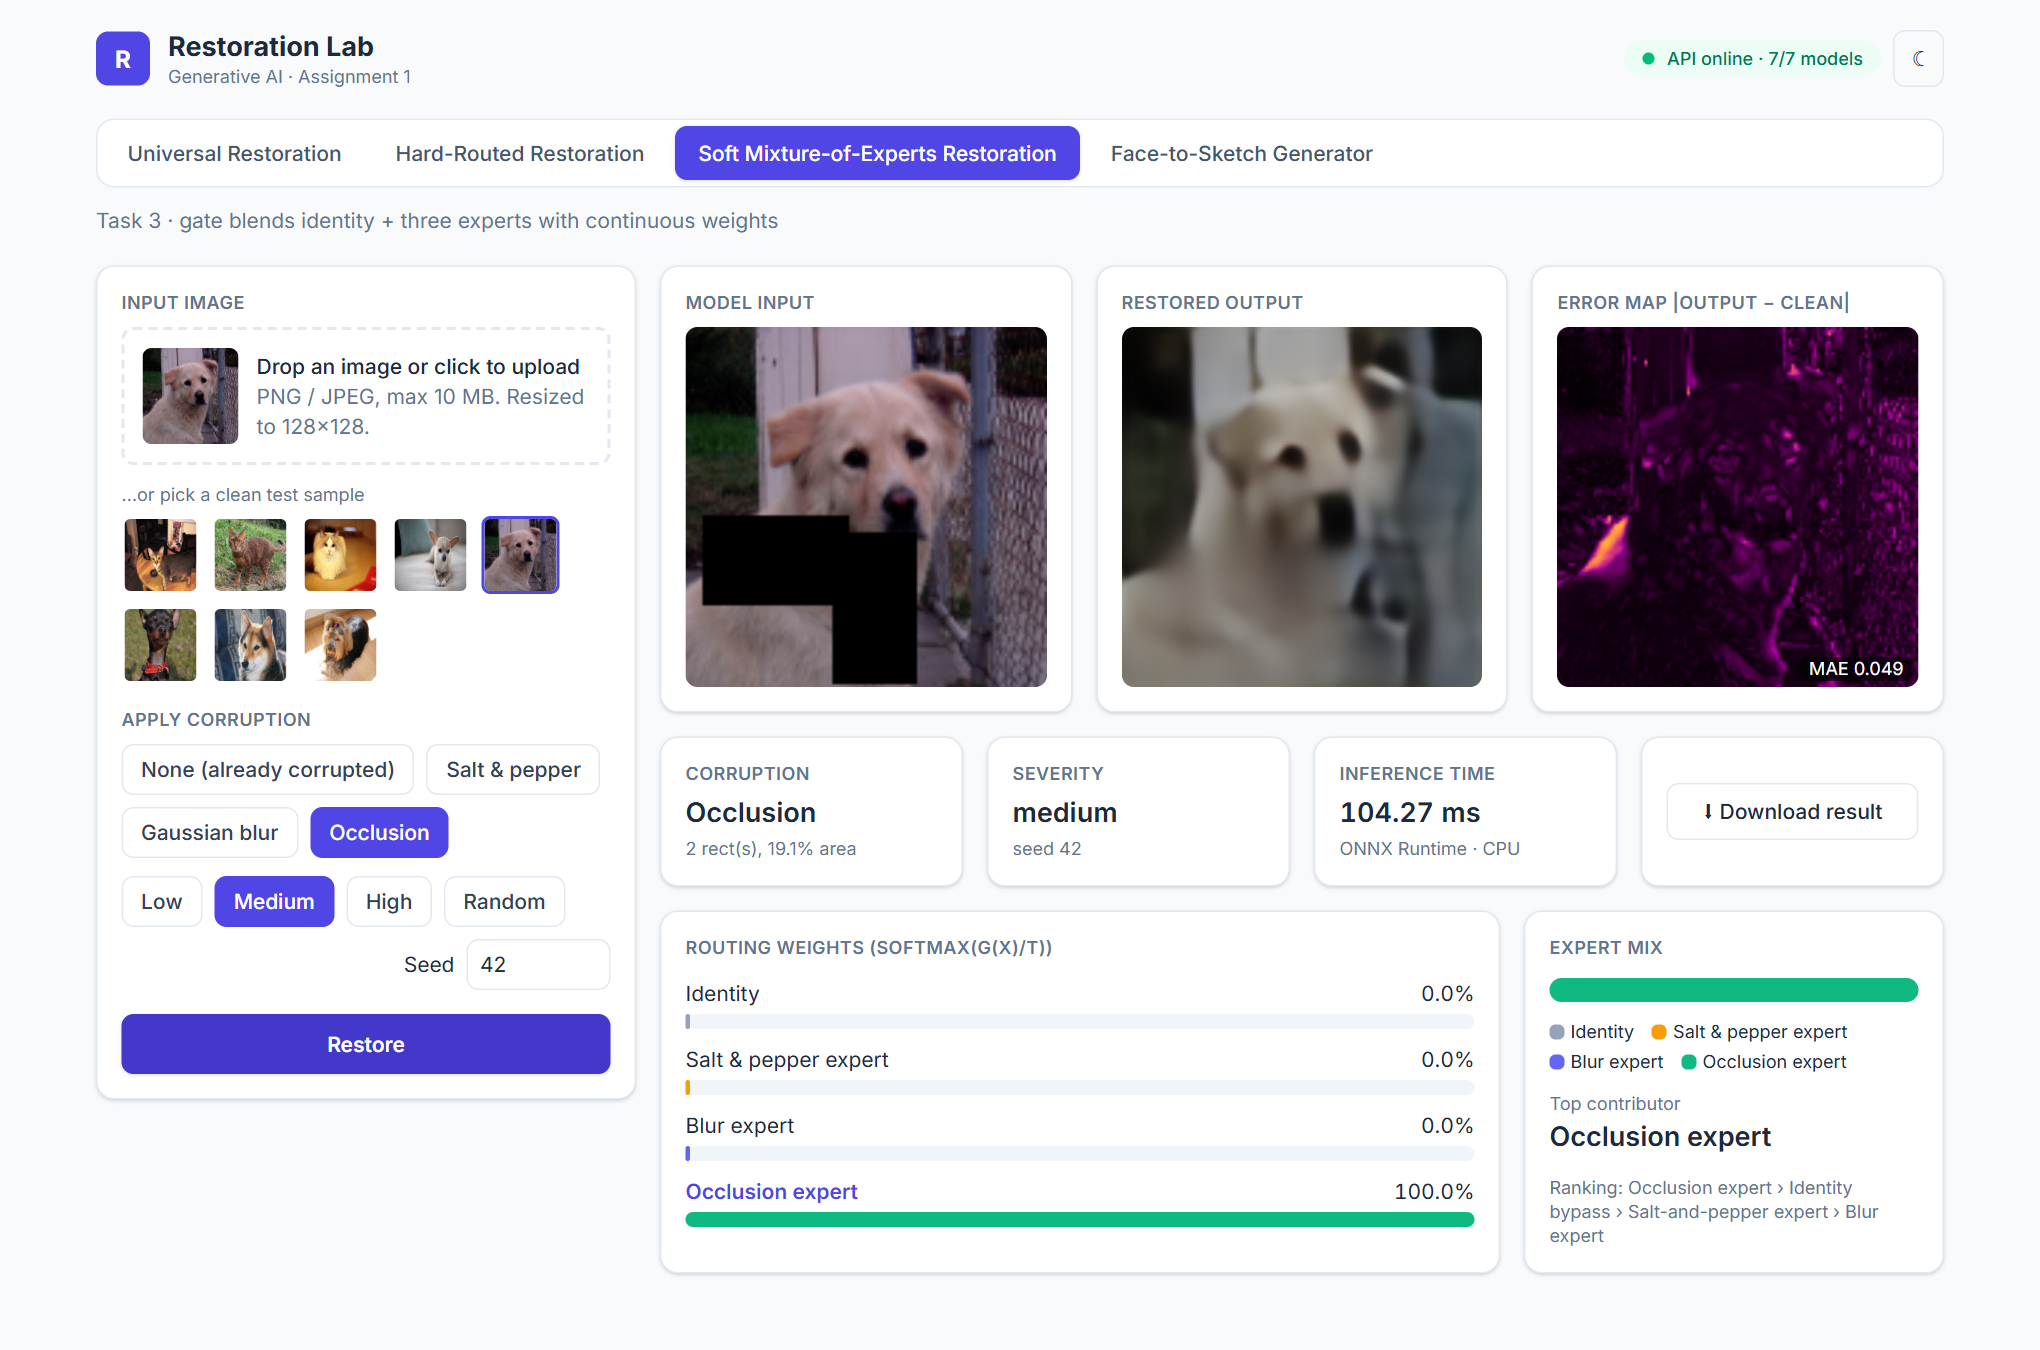
\includegraphics[width=0.42\textwidth]{app_moe.png}\hspace{2mm}
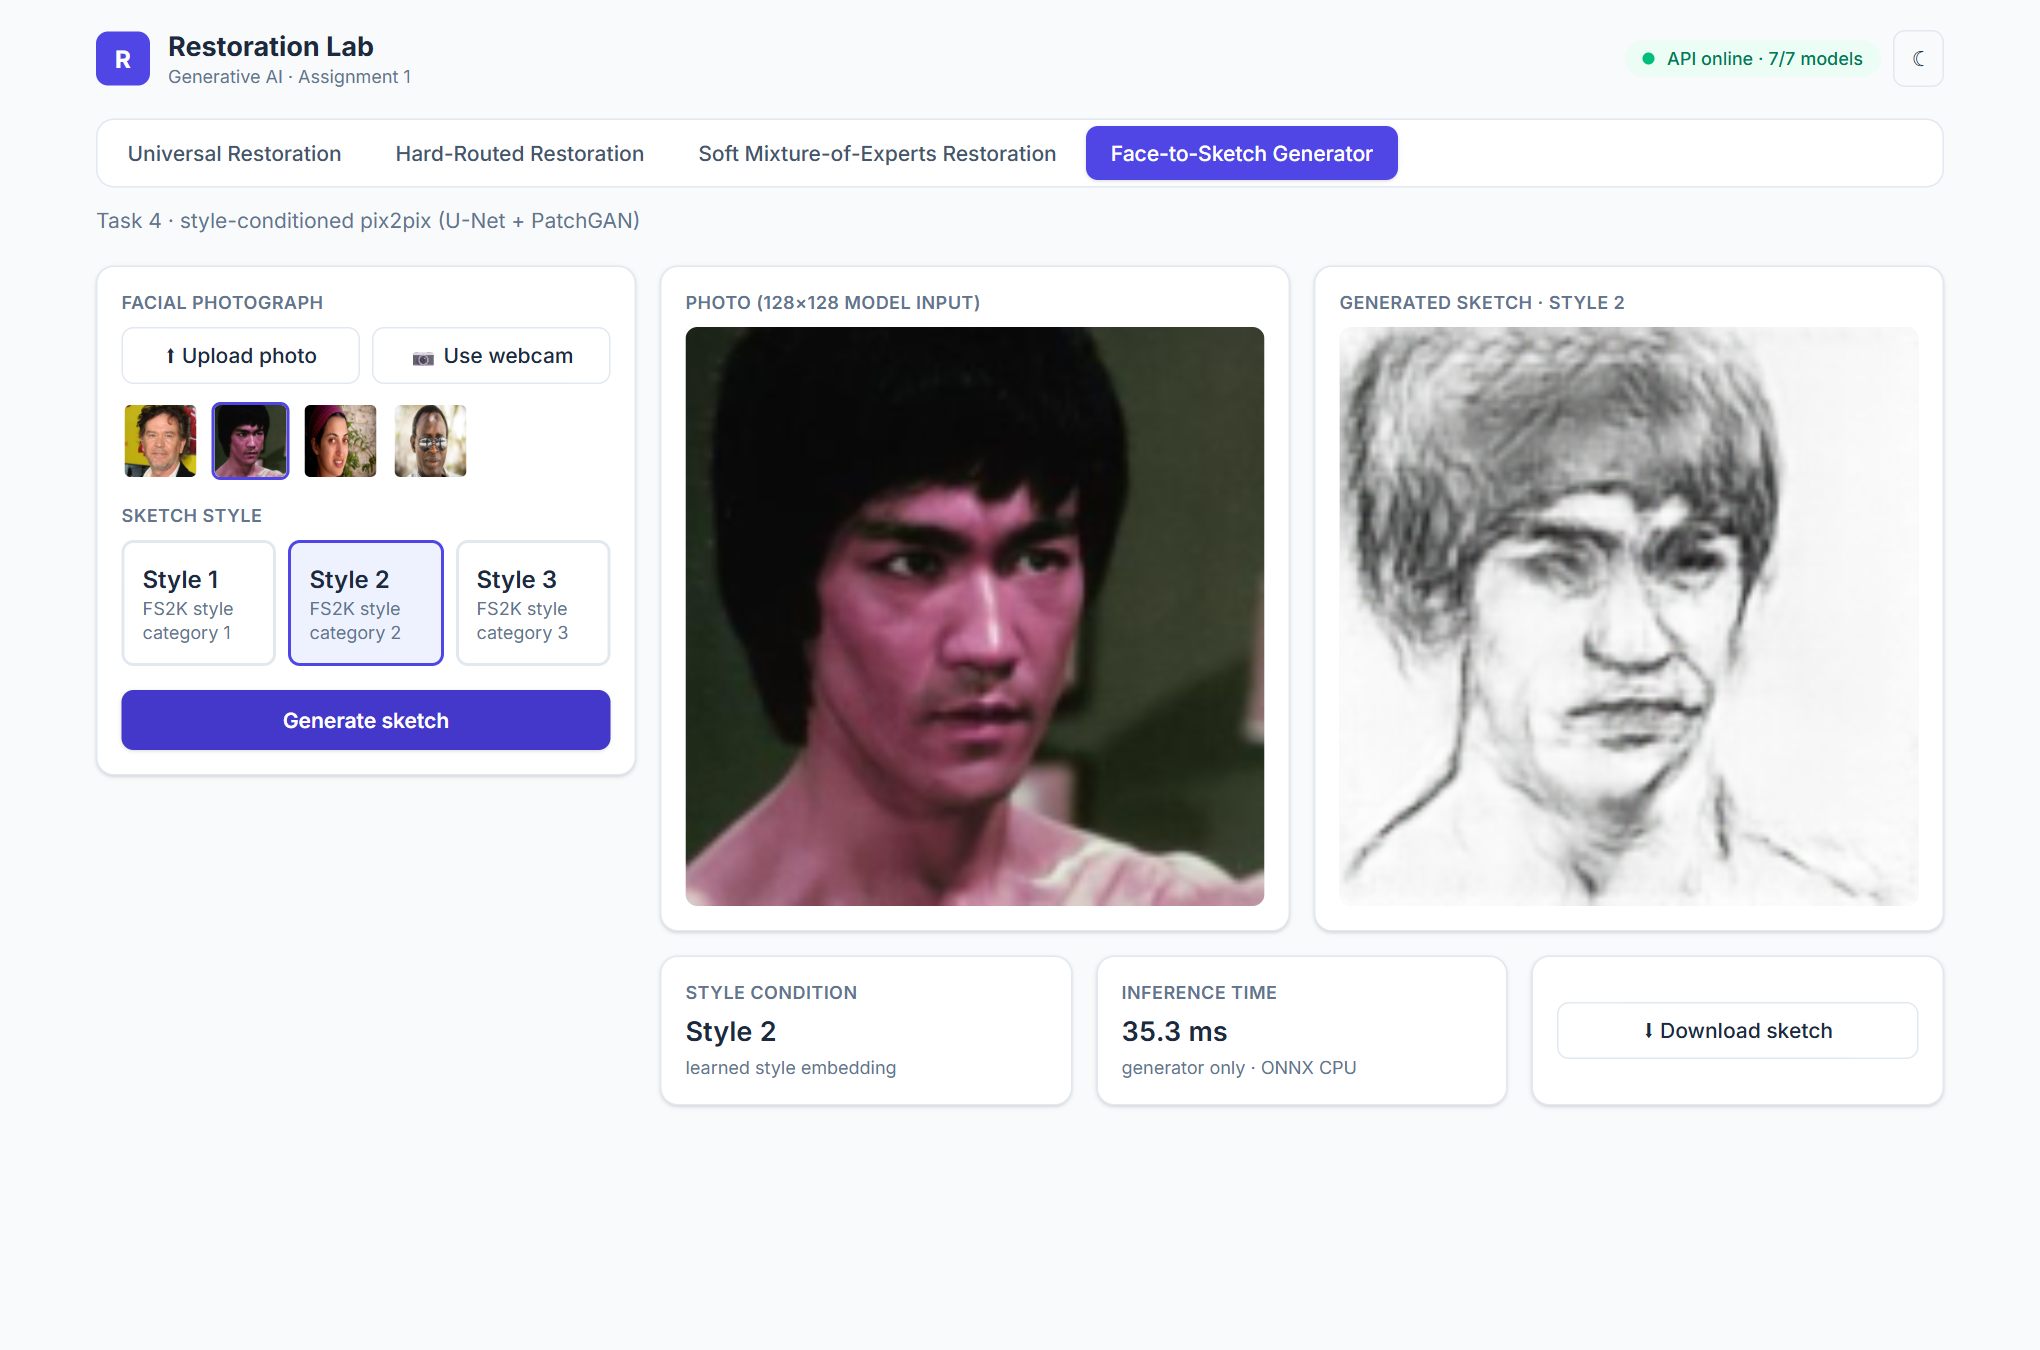
\includegraphics[width=0.42\textwidth]{app_sketch.png}
\caption{The deployed application with the trained models. Top left: Universal Restoration (salt-and-pepper applied at
runtime, input / output / error map, corruption settings, inference time, download). Top right: Hard-Routed Restoration
of an \emph{uploaded} photograph that is not part of the dataset samples (classifier probabilities, predicted
corruption, selected expert). Bottom left: Soft Mixture-of-Experts Restoration (all four routing weights, expert-mix bar,
top contributor). Bottom right: Face-to-Sketch Generator (style selection, side-by-side result, download; webcam capture
is available through the ``Use webcam'' button).}\label{fig:screens}
\end{figure*}

\begin{figure}[!htbp]
\centering
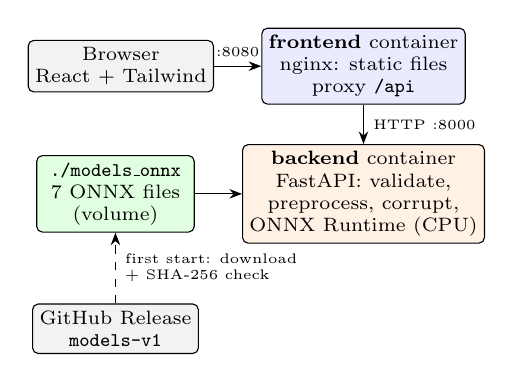
\begin{tikzpicture}[node distance=3mm]
\node[io, minimum width=20mm] (b) {Browser\\React + Tailwind};
\node[blk, fill=blue!8, right=6mm of b, minimum width=23mm] (n) {\textbf{frontend} container\\nginx: static files\\proxy \texttt{/api}};
\node[blk, fill=orange!10, below=5mm of n, minimum width=23mm] (f) {\textbf{backend} container\\FastAPI: validate,\\preprocess, corrupt,\\ONNX Runtime (CPU)};
\node[blk, fill=green!12, left=6mm of f, minimum width=20mm] (m) {\texttt{./models\_onnx}\\7 ONNX files\\(volume)};
\node[blk, fill=gray!10, below=9mm of m, minimum width=20mm] (r) {GitHub Release\\\texttt{models-v1}};
\draw[arr] (b)--node[above,font=\tiny]{:8080}(n);
\draw[arr] (n)--node[right,font=\tiny]{HTTP :8000}(f);
\draw[arr] (m)--(f);
\draw[arr, dashed] (r)--node[right,font=\tiny,align=left]{first start: download\\+ SHA-256 check}(m);
\end{tikzpicture}
\caption{Deployment: one \texttt{docker compose up -{}-build} starts both containers; the backend downloads and verifies
the models on its first start.}\label{fig:arch-app}
\end{figure}

\textbf{Design.} The interface was specified in Google Stitch (prompt in \texttt{docs/stitch/stitch\_prompt.md}):
one page with a status pill, four tabs named exactly as in the brief, an input card on the left and image panels,
statistics and task-specific cards on the right (Fig.~\ref{fig:stitch}). It was implemented in React with Tailwind
CSS (Fig.~\ref{fig:screens}).

\textbf{Architecture} (Fig.~\ref{fig:arch-app}). Docker Compose starts two containers. The \emph{frontend} container
builds the React app with Node~22 and serves it with nginx, which also proxies \texttt{/api/} to the backend. The
\emph{backend} container runs FastAPI with ONNX Runtime on the CPU. Its endpoints are \texttt{GET /health},
\texttt{/samples}, \texttt{/corruptions}, and \texttt{POST /corrupt}, \texttt{/restore/universal},
\texttt{/restore/hard}, \texttt{/restore/moe} and \texttt{/sketch}. Uploads are validated (image MIME type, decodable,
at most 10\,MB; errors 415/413/422), converted to RGB and resized to $128\times128$ exactly as in training; runtime
corruption calls the same module used for training. Responses contain the images (base64 PNG), inference time, the
classifier probabilities, predicted class and selected expert (Task~2) or the four MoE weights with their ranking
(Task~3). ONNX sessions are created lazily, and a missing model returns HTTP 503 with an explanation instead of
crashing.

\textbf{One-command start.} The evaluator runs \texttt{git clone}, then \texttt{docker compose up -{}-build}, and opens
\url{http://localhost:8080}. On its first start the backend downloads the seven ONNX files (330\,MB) from the GitHub
Release, verifies their SHA-256 checksums and writes them atomically to a mounted folder, so later starts reuse them;
download scripts for Windows and Linux are provided as an alternative. A GitHub Actions workflow reproduces the
evaluator's procedure on a clean Linux machine on every change: fresh clone, build, start, an end-to-end test of all
four workspaces and the upload validation through nginx, a restart, and the same test again. It passed, as did the
same test run locally against the real nginx.

\textbf{ONNX export.} All seven inference models were exported (opset 17) and compared with PyTorch on the same
inputs (Table~\ref{tab:onnx}); the largest absolute difference is $6.6\times10^{-6}$, far below the $10^{-4}$
tolerance. The MoE is exported as one graph that returns both the restored image and the four weights. On a laptop
CPU a request takes roughly 30--200\,ms after the first (model-loading) call.

\begin{table}[!htbp]
\centering\caption{ONNX models and PyTorch--ONNX Runtime parity}\label{tab:onnx}
\scriptsize\setlength{\tabcolsep}{4pt}
\begin{tabular}{@{}lrrc@{}}
\toprule
Model & Params & Size (MB) & Max abs.\ diff.\\
\midrule
T1 universal DAE & 5.39\,M & 20.6 & $2.4\times10^{-6}$\\
T2 classifier & 1.17\,M & 4.5 & $1.2\times10^{-7}$\\
T2 specialists (each) & 5.39\,M & 20.6 & $\le4.9\times10^{-6}$\\
T3 soft MoE (whole pipeline) & 17.34\,M & 66.2 & $2.6\times10^{-6}$\\
T4 generator & 42.12\,M & 160.7 & $6.6\times10^{-6}$\\
\bottomrule
\end{tabular}
\end{table}

% =====================================================================================================
\clearpage
\section{Limitations}\label{sec:limits}
(1)~The restoration models are limited by the 512-value spatial bottleneck: they improve heavily corrupted inputs but
degrade mild blur and clean images, and specialists do not outperform the universal model. The limited-skip ablation
shows a large gain but was not adopted. (2)~The Optuna budgets (10--15 short trials on half of the data) bias the
search towards fast-learning configurations, as the bottleneck choice shows; a multi-fidelity method (e.g.\
Hyperband) or longer trials would be more reliable. (3)~Joint MoE fine-tuning did not improve validation, so the
delivered MoE uses the warm-up checkpoint. (4)~Pixel metrics underrate stylised sketches, especially style~2; a
perceptual or FID-style evaluation would complement them, and FS2K test style labels are partly inconsistent.
(5)~All results come from single training runs (seed 42) without confidence intervals. (6)~Inputs are processed at
$128\times128$, so large uploaded photos lose detail before restoration.

\section{Conclusion}
We implemented, tuned, evaluated and deployed four generative models in one application. Explicit routing is
almost free of errors (99.6\% accuracy) and its main benefit is the identity bypass for clean images; soft routing
reaches the same accuracy while hedging on ambiguous low-severity occlusions, which gives the best occlusion SSIM.
The decisive factor for restoration quality, however, is architectural: the required compressed bottleneck caps all
three restoration systems at about 23\,dB, and one narrow skip connection removes most of that gap. For sketches, a
learned style embedding in both networks produces clearly different styles from the same photograph. The deployment
is reproducible from a fresh clone with one command and is tested automatically.

\textbf{Links.} Repository: \repourl. Trained models: \releaseurl. Experiment tracking: \wandburl.
Demonstration video: \youtubeurl.

% =====================================================================================================
% all figures are placed before the reference list
\clearpage
\begin{thebibliography}{99}\footnotesize
\bibitem{vincent2008} P.~Vincent, H.~Larochelle, Y.~Bengio, and P.-A.~Manzagol, ``Extracting and composing robust features with denoising autoencoders,'' in \emph{Proc. ICML}, 2008, pp.~1096--1103.
\bibitem{vincent2010} P.~Vincent, H.~Larochelle, I.~Lajoie, Y.~Bengio, and P.-A.~Manzagol, ``Stacked denoising autoencoders: Learning useful representations in a deep network with a local denoising criterion,'' \emph{J. Mach. Learn. Res.}, vol.~11, pp.~3371--3408, 2010.
\bibitem{mao2016} X.-J.~Mao, C.~Shen, and Y.-B.~Yang, ``Image restoration using very deep convolutional encoder-decoder networks with symmetric skip connections,'' in \emph{Proc. NIPS}, 2016, pp.~2802--2810.
\bibitem{zhang2017} K.~Zhang, W.~Zuo, Y.~Chen, D.~Meng, and L.~Zhang, ``Beyond a Gaussian denoiser: Residual learning of deep CNN for image denoising,'' \emph{IEEE Trans. Image Process.}, vol.~26, no.~7, pp.~3142--3155, 2017.
\bibitem{wang2004} Z.~Wang, A.~C.~Bovik, H.~R.~Sheikh, and E.~P.~Simoncelli, ``Image quality assessment: From error visibility to structural similarity,'' \emph{IEEE Trans. Image Process.}, vol.~13, no.~4, pp.~600--612, 2004.
\bibitem{zhao2017} H.~Zhao, O.~Gallo, I.~Frosio, and J.~Kautz, ``Loss functions for image restoration with neural networks,'' \emph{IEEE Trans. Comput. Imaging}, vol.~3, no.~1, pp.~47--57, 2017.
\bibitem{jacobs1991} R.~A.~Jacobs, M.~I.~Jordan, S.~J.~Nowlan, and G.~E.~Hinton, ``Adaptive mixtures of local experts,'' \emph{Neural Comput.}, vol.~3, no.~1, pp.~79--87, 1991.
\bibitem{shazeer2017} N.~Shazeer, A.~Mirhoseini, K.~Maziarz, A.~Davis, Q.~Le, G.~Hinton, and J.~Dean, ``Outrageously large neural networks: The sparsely-gated mixture-of-experts layer,'' in \emph{Proc. ICLR}, 2017.
\bibitem{fedus2022} W.~Fedus, B.~Zoph, and N.~Shazeer, ``Switch transformers: Scaling to trillion parameter models with simple and efficient sparsity,'' \emph{J. Mach. Learn. Res.}, vol.~23, no.~120, pp.~1--39, 2022.
\bibitem{goodfellow2014} I.~Goodfellow, J.~Pouget-Abadie, M.~Mirza, B.~Xu, D.~Warde-Farley, S.~Ozair, A.~Courville, and Y.~Bengio, ``Generative adversarial nets,'' in \emph{Proc. NIPS}, 2014, pp.~2672--2680.
\bibitem{mirza2014} M.~Mirza and S.~Osindero, ``Conditional generative adversarial nets,'' arXiv:1411.1784, 2014.
\bibitem{isola2017} P.~Isola, J.-Y.~Zhu, T.~Zhou, and A.~A.~Efros, ``Image-to-image translation with conditional adversarial networks,'' in \emph{Proc. CVPR}, 2017, pp.~1125--1134.
\bibitem{ronneberger2015} O.~Ronneberger, P.~Fischer, and T.~Brox, ``U-Net: Convolutional networks for biomedical image segmentation,'' in \emph{Proc. MICCAI}, 2015, pp.~234--241.
\bibitem{ulyanov2016} D.~Ulyanov, A.~Vedaldi, and V.~Lempitsky, ``Instance normalization: The missing ingredient for fast stylization,'' arXiv:1607.08022, 2016.
\bibitem{fan2022} D.-P.~Fan, Z.~Huang, P.~Zheng, H.~Liu, X.~Qin, and L.~Van Gool, ``Facial-sketch synthesis: A new challenge,'' \emph{Mach. Intell. Res.}, vol.~19, no.~4, pp.~257--287, 2022.
\bibitem{wang2009} X.~Wang and X.~Tang, ``Face photo-sketch synthesis and recognition,'' \emph{IEEE Trans. Pattern Anal. Mach. Intell.}, vol.~31, no.~11, pp.~1955--1967, 2009.
\bibitem{parkhi2012} O.~M.~Parkhi, A.~Vedaldi, A.~Zisserman, and C.~V.~Jawahar, ``Cats and dogs,'' in \emph{Proc. CVPR}, 2012, pp.~3498--3505.
\bibitem{akiba2019} T.~Akiba, S.~Sano, T.~Yanase, T.~Ohta, and M.~Koyama, ``Optuna: A next-generation hyperparameter optimization framework,'' in \emph{Proc. ACM SIGKDD}, 2019, pp.~2623--2631.
\bibitem{bergstra2011} J.~Bergstra, R.~Bardenet, Y.~Bengio, and B.~K\'egl, ``Algorithms for hyper-parameter optimization,'' in \emph{Proc. NIPS}, 2011, pp.~2546--2554.
\bibitem{loshchilov2019} I.~Loshchilov and F.~Hutter, ``Decoupled weight decay regularization,'' in \emph{Proc. ICLR}, 2019.
\bibitem{kingma2015} D.~P.~Kingma and J.~Ba, ``Adam: A method for stochastic optimization,'' in \emph{Proc. ICLR}, 2015.
\bibitem{odena2016} A.~Odena, V.~Dumoulin, and C.~Olah, ``Deconvolution and checkerboard artifacts,'' \emph{Distill}, 2016. [Online]. Available: \url{https://distill.pub/2016/deconv-checkerboard/}
\bibitem{wandb} L.~Biewald, ``Experiment tracking with Weights and Biases,'' 2020. [Online]. Available: \url{https://www.wandb.com/}
\bibitem{onnxruntime} ONNX Runtime developers, ``ONNX Runtime,'' 2021. [Online]. Available: \url{https://onnxruntime.ai/}
\end{thebibliography}

% =====================================================================================================
\appendices
\section{Use of AI Tools}
AI assistants were used as permitted by the brief. Table~\ref{tab:ai} lists the tools, what they were used for and how
their output was checked; the full log is \texttt{docs/ai\_use.md} in the repository.

\begin{table}[h]
\centering\caption{AI-tool use and verification}\label{tab:ai}
\scriptsize\setlength{\tabcolsep}{2pt}
\begin{tabular}{@{}p{0.17\columnwidth}p{0.36\columnwidth}p{0.43\columnwidth}@{}}
\toprule
Tool & Used for & How the output was verified or corrected\\
\midrule
Claude (Cowork) & Breaking down the brief, project plan, repository scaffold & Checked requirement by requirement against the assignment PDF\\
Claude & Corruption module, data pipeline, manifests & Unit tests (parameter ranges, occlusion union area, determinism from seed); visual sanity grid\\
Claude Code & Models, training engines, Optuna studies, evaluation, ONNX export & CPU smoke tests on synthetic data; ONNX parity check ($<10^{-4}$); metrics cross-checked against per-item CSV files\\
Claude Code (GPU PC) & Data download, running the studies and training, efficiency fixes, ablations & Each change measured before adoption (\texttt{cudnn.benchmark}, data-loader workers); mirror data asserted equal to the official image lists; failures (memory, power loss) diagnosed from logs and resumed from checkpoints\\
Claude Code & FastAPI backend, React frontend, Docker files, model auto-download, CI workflow & End-to-end test of all endpoints through nginx; browser test of every workspace with an unseen uploaded image; GitHub Actions fresh-clone \texttt{docker compose} test\\
Claude Code & Figures and first draft of this report & Every number taken from the result files in \texttt{results/}; text reviewed and edited by the author\\
\bottomrule
\end{tabular}
\end{table}

\end{document}
